\documentclass[12pt]{article}

% ── Packages ──────────────────────────────────────────────────────────────────
\usepackage{graphicx}
\usepackage{amsmath}
\usepackage{amssymb}
\usepackage{hyperref}
\usepackage{geometry}
\usepackage{caption}
\usepackage{subcaption}
\usepackage{listings}
\usepackage{cite}
\usepackage{longtable}
\usepackage{booktabs}
\usepackage{array}
\usepackage{xcolor}
\usepackage{colortbl}
\usepackage{multirow}
\usepackage{setspace}
\usepackage{fancyhdr}
\setlength{\headheight}{15pt}
\usepackage{titlesec}
\usepackage{enumitem}
\usepackage{float}
\usepackage{algorithm}
\usepackage{algpseudocode}
\usepackage{tikz}
\usepackage{pgfplots}
\pgfplotsset{compat=1.18}
\usepackage{mdframed}
\usepackage{tcolorbox}
\usepackage{microtype}
\usepackage{parskip}
\usepackage{tabularx}
\usepackage{ragged2e}

% ── Page Layout ───────────────────────────────────────────────────────────────
\geometry{a4paper, margin=1in}
\captionsetup{font=small, labelfont=bf}
\onehalfspacing

% ── Header / Footer ───────────────────────────────────────────────────────────
\pagestyle{fancy}
\fancyhf{}
\rhead{\small\textit{Heuristic Search Algorithms to Optimize NLP Query}}
\lhead{\small\textit{Daud Ahmed --- 202402480}}
\cfoot{\thepage}
\renewcommand{\headrulewidth}{0.4pt}

% ── Colours ───────────────────────────────────────────────────────────────────
\definecolor{headerblue}{RGB}{31,56,100}
\definecolor{rowalt}{RGB}{235,243,251}
\definecolor{rowhigh}{RGB}{255,242,204}
\definecolor{codegreen}{rgb}{0,0.45,0}
\definecolor{codegray}{rgb}{0.4,0.4,0.4}
\definecolor{codebg}{RGB}{248,248,248}
\definecolor{myblue}{RGB}{31,56,100}
\definecolor{alertred}{RGB}{200,40,40}

% ── Code listings ─────────────────────────────────────────────────────────────
\lstset{
	basicstyle=\ttfamily\small,
	backgroundcolor=\color{codebg},
	breaklines=true,
	commentstyle=\color{codegreen}\itshape,
	keywordstyle=\color{blue}\bfseries,
	stringstyle=\color{orange!80!black},
	showstringspaces=false,
	frame=single,
	rulecolor=\color{gray!40},
	numbers=left,
	numberstyle=\tiny\color{codegray},
	tabsize=4,
	xleftmargin=1.5em
}

% ── Hyperlink setup ───────────────────────────────────────────────────────────
\hypersetup{
	colorlinks=true,
	linkcolor=blue!70!black,
	citecolor=blue!60!black,
	urlcolor=blue!70!black
}

% ── Column types ─────────────────────────────────────────────────────────────
\newcolumntype{C}[1]{>{\centering\arraybackslash}p{#1}}
\newcolumntype{L}[1]{>{\raggedright\arraybackslash}p{#1}}
\newcolumntype{R}[1]{>{\raggedleft\arraybackslash}p{#1}}

\newcommand{\hdrcel}[1]{\cellcolor{headerblue}\textcolor{white}{\textbf{#1}}}

% ── Insight box ───────────────────────────────────────────────────────────────
\newenvironment{insightbox}[1]{%
	\begin{tcolorbox}[colback=rowalt, colframe=myblue, title=\textbf{#1},
		fonttitle=\small\color{white}, coltitle=white,
		colbacktitle=myblue, boxrule=0.5pt]
	}{%
	\end{tcolorbox}
}

% =============================================================================
\begin{document}
	% =============================================================================
	
	% ── Title Page ────────────────────────────────────────────────────────────────
	\begin{titlepage}
		\centering
		
\includegraphics[width=0.3\textwidth]{STFX_Logo.png}\par
		\vspace{1cm}
		{\Huge\bfseries St.\ Francis Xavier University\par}
		\vspace{0.5cm}
		{\LARGE Heuristic Search Algorithms to\\[0.4cm] Optimize NLP Query\par}
		\vspace{1.5cm}
		{\Large Dr.\ Hao Cai\par}
		\vspace{0.3cm}
		{\large CSCI 564 - Processing \& Heuristic Search\par}
		\vspace{2cm}
		\begin{tabular}{c}
			{\large Daud Ahmed}\\
			{\large 202402480 - x2024ehm@stfx.ca}\\[0.8cm]
			\url{https://github.com/DaudAhmed008/optimize-nlp-query-using-heuristic-search}
		\end{tabular}
	\end{titlepage}
	
	\newpage
	\tableofcontents
	\listoffigures
	\listoftables
	\newpage
	
	% =============================================================================
	\section{Introduction}
	% =============================================================================
	
	\subsection{Background and Motivation}
	
	When a chatbot replies to your message, a summariser condenses a document, or your phone predicts the next word you are about to type, a language model is solving the same problem on repeat: given the text so far, which token comes next? The model itself does not pick the answer. It produces a probability distribution over tens of thousands of candidates, and a separate mechanism, the \emph{decoding algorithm}, decides which candidates actually make it into the output. Most NLP courses treat decoding as an afterthought. The experiments in this report show that it deserves far more attention than that.

	The question driving this project is narrow but consequential: if the language model stays the same and only the decoding algorithm changes, how different can the generated text get? The answer, confirmed across every experiment reported here, is \emph{very} different. The same GPT-2 model, given the same prompt, can produce anything from a 7-word sentence fragment to a 135-word paragraph depending on which algorithm navigates the probability space.
	
	GPT-2~\cite{radford2019gpt2} is the model used throughout. It is a 117-million-parameter transformer trained by OpenAI on a large English web corpus. It would be fair to call it dated by 2025 standards, but that is partly the point. It is small enough to run dozens of experiments on a CPU in an afternoon. It is large enough to generate syntactically correct, contextually coherent text. It is well-documented, widely available, and carries no API restrictions. When the goal is to isolate the effect of the decoding algorithm from everything else, those properties matter more than raw capability.
	
	Version~1.0 of this project compared three algorithms (Greedy, Beam Search, and A$^*$) on a single prompt with a 50-token limit. That version exposed three problems. The A$^*$ heuristic had a design flaw: it scored short sequences so favourably that the algorithm would stop after producing just 7 words. Three algorithms was too few to cover the range of decoding philosophies in the literature. And a single prompt made it impossible to tell whether the results reflected the algorithms or the idiosyncrasies of that particular prompt. Version~3.0 addresses all three.
	
	\subsection{What Was Added in Version 3.0}
	
	Four new algorithms were added for this version:
	
	\textbf{BFS (Breadth-First Search)} was added as a classical search baseline per the course instructor's suggestion. It explores all candidates at each depth before moving deeper, with \texttt{branch\_factor=3} and \texttt{max\_depth=15} to stay tractable, then extends the best sequence greedily.
	
	\textbf{Hill Climbing Search} starts from a Greedy-generated sequence and tries to improve it by swapping individual tokens for better alternatives. Version~3.0 improves it with multi-token substitution (targeting the 5 worst-scoring positions per pass), increased \texttt{top\_k} from 5 to 10, \texttt{max\_iter} from 3 to 5, and 3 random restarts from temperature-sampled seeds. The course instructor suggested testing it, and the question of whether it actually beats Greedy Search turned out to have a surprisingly definitive answer.
	
	\textbf{Contrastive Search}~\cite{su2022contrastive} won Best Paper at EMNLP 2022. Instead of following high-probability paths (the way Greedy and Beam Search do), it penalises tokens that are semantically similar to what has already been generated, using cosine similarity in GPT-2's embedding space. The claim is that this directly addresses neural text degeneration, the repetitive, circular output that plagued earlier decoding methods. That claim is worth testing.
	
	\textbf{Simulated Annealing} borrows from metallurgy. At high temperature it samples broadly from the probability distribution; as temperature drops, it gradually converges toward greedy behaviour. The question is whether the creative, non-deterministic output it produces can compete on standard quality metrics with the deterministic algorithms.
	
	The A$^*$ heuristic was also redesigned. Version~1.0 used raw average log-probability as the estimate $h(n)$, which penalised long sequences by accumulating negative values. Version~3.0 computes the heuristic from the \emph{same} forward pass used for expansion (cutting GPT-2 calls roughly in half), increases $\alpha$ from 0.7 to 0.8, and adds a minimum-length penalty of 20 tokens to combat short-output bias.
	
	\subsection{Why These Seven Algorithms?}
	
	The seven algorithms were chosen to cover the main philosophical approaches to decoding:
	
	\begin{itemize}[leftmargin=*]
		\item \textbf{Pure exploitation} (Greedy Search): always picks the single highest-probability token, never looks sideways.
		\item \textbf{Bounded multi-path search} (Beam Search): maintains a fixed-width frontier, balancing exploration against exploitation.
		\item \textbf{Exhaustive breadth-first exploration} (BFS): expands all candidates at each depth before moving deeper, providing a classical search baseline.
		\item \textbf{Iterative local refinement} (Hill Climbing): generates a complete output first, then tries to improve it token by token.
		\item \textbf{Global priority-guided search} (A$^*$ Search): maintains a globally-sorted frontier using a heuristic estimate of remaining quality.
		\item \textbf{Anti-degeneration decoding} (Contrastive Search): penalises semantic repetition directly in embedding space.
		\item \textbf{Temperature-scheduled stochastic sampling} (Simulated Annealing): controls exploration through a cooling schedule.
	\end{itemize}
	
	Each approach has been proposed seriously in the literature and deployed in real systems. Comparing all seven in one study, on the same model and prompts, provides a broader picture than any pairwise comparison could.
	
	\subsection{Structure of the Report}
	
	Section~\ref{sec:litreview} covers the theoretical background for the seven algorithms and three evaluation metrics. Section~\ref{sec:problem} states the research questions and describes the experimental challenges. Section~\ref{sec:method} details the implementations, including pseudocode and parameter choices. Section~\ref{sec:results} presents the full empirical results with per-prompt breakdowns. Section~\ref{sec:discussion} interprets the results, including an explanation of A$^*$'s paradoxical dominance despite producing very short outputs. Section~\ref{sec:threats} discusses threats to validity. Section~\ref{sec:conclusion} summarises findings and outlines future work. Appendix~\ref{app:outputs} contains sample generated text from all seven algorithms across all six prompts.
	
	% =============================================================================
	\section{Literature Review}
	\label{sec:litreview}
	% =============================================================================
	
	\subsection{The Text Generation Problem}
	
	Text generation requires producing a sequence of tokens $t_1, t_2, \ldots, t_L$ that is coherent, fluent, and relevant to a given prompt $p$. A language model defines a conditional probability distribution $P(t_i \mid p, t_1, \ldots, t_{i-1})$ over the vocabulary $\mathcal{V}$ at each position $i$. The ideal sequence maximises the joint probability:
	
	\begin{equation}
		\hat{T} = \operatorname{argmax}_{t_1,\ldots,t_L \in \mathcal{V}^L}
		\prod_{i=1}^{L} P(t_i \mid p, t_1, \ldots, t_{i-1})
		\label{eq:argmax}
	\end{equation}
	
	Finding this optimum is intractable. For GPT-2's vocabulary of 50,257 tokens and $L=150$, the search space contains more than $10^{700}$ candidate sequences. Every algorithm in this study is an approximation to~\eqref{eq:argmax}, and each makes different trade-offs between quality and efficiency.
	
	\subsection{GPT-2: Architecture and Properties}
	
	GPT-2~\cite{radford2019gpt2} is a decoder-only Transformer~\cite{vaswani2017attention} trained autoregressively on the WebText dataset. The base model has 12 transformer blocks, 12 attention heads per block, a hidden dimension of 768, and 117~million parameters in total. Each forward pass produces a logit vector $z \in \mathbb{R}^{|\mathcal{V}|}$, converted to probabilities via softmax:
	
	\begin{equation}
		P(t = v \mid \text{context}) = \frac{\exp(z_v)}{\sum_{v' \in \mathcal{V}} \exp(z_{v'})}
		\label{eq:softmax}
	\end{equation}
	
	GPT-2 tokenises text using byte-pair encoding (BPE), so its vocabulary consists of subword units rather than whole words. This creates a practical wrinkle for evaluation: ``word count'' and ``token count'' are not the same thing. The output lengths in this study are reported in words (whitespace-delimited tokens) for readability, while the algorithms themselves operate on BPE tokens internally.
	
	Holtzman et al.~\cite{holtzman2020curious} documented a phenomenon they called \emph{neural text degeneration}: greedy and beam decoding with models like GPT-2 frequently produce repetitive, circular, or topically drifting text. Their core observation is that sequences with high probability under the model's distribution are not necessarily high quality from a human perspective. This is the problem that Contrastive Search and Simulated Annealing were specifically designed to address.
	
	\subsection{Heuristic Search in AI and NLP}
	
	Heuristic search is a classical topic in artificial intelligence~\cite{russellnorvig2020ai}. The general framework involves a state space (here, partial token sequences), operators (appending a token), a cost function (negative log-probability), and a heuristic function $h(n)$ that estimates the remaining cost to reach a goal state from state $n$.
	
	The theoretical appeal of A$^*$ Search is its optimality guarantee: if $h(n)$ never overestimates the true cost to goal (i.e., is \emph{admissible}), A$^*$ is guaranteed to find the optimal solution~\cite{hart1968astar}. Applying this guarantee to text generation, however, runs into three obstacles: (a) there is no clearly defined goal state; (b) the cost function is computed incrementally, one token at a time; and (c) evaluating the true remaining cost would require generating every possible continuation. The heuristic used in this study is an approximation, not a formally admissible one, so A$^*$'s optimality guarantee does not hold here.
	
	\subsection{Decoding Algorithms: Detailed Review}
	
	\subsubsection{Greedy Search}
	\label{sec:greedy_theory}
	
	Greedy Search is the simplest decoding strategy. At each step $i$, it picks the single most probable token:
	
	\begin{equation}
		t_i^* = \operatorname{argmax}_{v \in \mathcal{V}} P(v \mid p, t_1, \ldots, t_{i-1})
		\label{eq:greedy}
	\end{equation}
	
	The output is deterministic: same input, same output, every time. Time complexity is $\mathcal{O}(L \cdot |\mathcal{V}|)$ for $L$ steps, dominated by the softmax computation at each step. Memory complexity is $\mathcal{O}(L)$.
	
	The well-known weakness is the local optimum problem. A token that maximises $P(t_i \mid \cdot)$ at step $i$ can steer subsequent probabilities toward poor tokens, producing a final sequence with lower joint probability than one that made a slightly worse choice at step $i$. This is not a bug; it is a structural consequence of greedy local search~\cite{russellnorvig2020ai}.
	
	In practice, Greedy Search with GPT-2 tends to produce repetitive text. The model's training objective (next-token prediction on web text) assigns high probability to common transition patterns. Once the greedy decoder locks onto one of these patterns, it loops.
	
	\subsubsection{Beam Search}
	\label{sec:beam_theory}
	
	Beam Search tackles the local optimum problem by maintaining $B$ partial sequences (the ``beam'') at each step. At step $i$, each of the $B$ hypotheses is expanded by all $|\mathcal{V}|$ possible next tokens, producing $B \cdot |\mathcal{V}|$ candidates scored by cumulative log-probability:
	
	\begin{equation}
		\mathrm{score}(t_1, \ldots, t_i) = \sum_{j=1}^{i} \log P(t_j \mid p, t_1, \ldots, t_{j-1})
		\label{eq:beam_score}
	\end{equation}
	
	The top $B$ candidates survive to the next step. After $L$ steps, the highest-scoring sequence is returned.
	
	Beam Search is the workhorse of production NLP. Google Translate, Facebook's M2M-100, and the vast majority of seq2seq summarisation models published in the last decade all rely on it~\cite{cho2014rnnencoder, see2017pointer}. The reasons are practical: it is fast in batched implementations, deterministic and reproducible, and it consistently produces more coherent text than Greedy Search for similar computational cost.
	
	The known limitation is a tendency toward bland, high-probability output. Meister et al.~\cite{meister2020beam} showed that increasing beam width can paradoxically \emph{decrease} output quality on some metrics, because the algorithm over-optimises cumulative log-probability at the expense of diversity. The no-repeat-bigram constraint used in this study is a common workaround that suppresses the most obvious repetition.
	
	\subsubsection{Hill Climbing Search}
	\label{sec:hillclimb_theory}
	
	Hill Climbing is an iterative improvement strategy. It starts from a complete solution (here, a Greedy-generated sequence) and scans through it, replacing individual tokens with alternatives that improve a quality measure. The quality measure used here is the average log-probability of the full sequence:
	
	\begin{equation}
		\mathrm{quality}(t_1, \ldots, t_L) = \frac{1}{L}\sum_{j=1}^{L}
		\log P(t_j \mid p, t_1, \ldots, t_{j-1})
		\label{eq:hill_quality}
	\end{equation}
	
	Because the algorithm only accepts substitutions that strictly increase this score, and the score is bounded above by zero, termination is guaranteed. What is \emph{not} guaranteed is a global optimum: the algorithm finds a local optimum of~\eqref{eq:hill_quality} from which no single-token swap can improve the score.
	
	Hill Climbing was included for two reasons. First, it represents a qualitatively different paradigm: post-hoc refinement rather than guided generation. Second, the course instructor suggested it, and the empirical question of whether it improves over Greedy turned out to be worth answering.
	
	\subsubsection{A* Search}
	\label{sec:astar_theory}
	
	A$^*$ Search~\cite{hart1968astar} generalises Greedy and Beam Search by using a global priority queue. Every partial sequence in the frontier is ranked by:
	
	\begin{equation}
		f(n) = g(n) + h(n)
		\label{eq:astar_f}
	\end{equation}
	
	where $g(n)$ is the cumulative log-probability of the sequence so far, and $h(n)$ is a heuristic estimate of the remaining quality. At each step, the algorithm expands whichever partial sequence has the highest $f(n)$, regardless of its generation depth. Beam Search, by contrast, processes all hypotheses at the same depth in lock-step. This is the key structural difference.
	
	The practical consequence is that A$^*$ can return to a short, high-scoring sequence and extend it further, even after exploring longer alternatives. This global priority structure makes A$^*$ theoretically more flexible than Beam Search, but also more expensive, because the priority queue can grow large.
	
	\paragraph{The heuristic function.}
	Version~1.0 defined $h(n)$ as the average log-probability of the current partial sequence. This was a mistake. Log-probabilities are negative and accumulate as the sequence grows, so $g(n)$ strictly decreases. The average $h(n) = g(n) / |n|$ also tends to decrease with length (GPT-2's distribution spreads more as context grows). The priority queue therefore consistently ranked short, high-confidence sequences above longer ones, causing A$^*$ to terminate after just 7 words.
	
	Version~3.0 uses the length-normalised heuristic from Google's GNMT system~\cite{wu2016gnmt}, computed from the \emph{same} forward pass used for expansion (eliminating the separate heuristic call and cutting GPT-2 forward passes roughly in half):
	
	\begin{equation}
		h(n) = \frac{\sum_{i=1}^{T} \log p(t_i)}{T^{\,\alpha}}, \qquad \alpha = 0.8
		\label{eq:heuristic}
	\end{equation}
	
	Dividing by $T^{0.8}$ softens the length penalty. A minimum-length penalty is also applied: sequences shorter than 20 tokens receive an additional score reduction to discourage premature termination. Whether these fixes are sufficient is tested experimentally; as Section~\ref{sec:length} shows, the fix is partial.
	
	\subsubsection{Contrastive Search}
	\label{sec:contrastive_theory}
	
	Contrastive Search~\cite{su2022contrastive} diagnoses text degeneration differently. Rather than blaming the search procedure for chasing high-probability paths, it argues the problem is semantic: degenerate text consists of tokens that are semantically similar to tokens already in the sequence, creating circular content even when the surface forms differ. The fix is to penalise this semantic similarity directly.
	
	At each step, the top-$k$ most probable tokens are identified. Each candidate $v$ is scored by:
	
	\begin{equation}
		\mathrm{score}(v) = (1-\alpha) \cdot P(v \mid \text{context})
		- \alpha \cdot \max_{t_j \in \text{prev}} \cos\bigl(\mathbf{e}(v), \mathbf{e}(t_j)\bigr)
		\label{eq:contrastive}
	\end{equation}
	
	where $\mathbf{e}(v)$ is the embedding of token $v$ from GPT-2's embedding matrix, $\mathbf{e}(t_j)$ is the embedding of a previously generated token, and $\alpha \in [0,1]$ controls the diversity-fluency trade-off. At $\alpha = 0$, this reduces to Greedy Search. At $\alpha = 1$, only diversity matters.
	
	With $\alpha = 0.6$, the algorithm allocates 40\% of its attention to model probability and 60\% to avoiding semantic self-repetition. Su and Peng~\cite{su2023contrastive_tacl} reported that this produces measurably less repetitive, more coherent text than Beam Search on both GPT-2 and GPT-3 benchmarks.
	
	\subsubsection{Simulated Annealing}
	\label{sec:sa_theory}
	
	Simulated Annealing~\cite{kirkpatrick1983annealing} borrows its metaphor from metallurgy: slowly cooling molten metal gives atoms time to settle into low-energy crystalline configurations, while rapid cooling traps them in disordered states. In search terms, high temperature early on permits broad exploration (including suboptimal moves), while low temperature late in the process forces convergence toward the best available option.
	
	For text generation, temperature $T$ is applied by scaling the logits before softmax:
	
	\begin{equation}
		P_T(v \mid \text{context}) = \frac{\exp(z_v / T)}{\sum_{v'} \exp(z_{v'} / T)}
		\label{eq:sa_prob}
	\end{equation}
	
	When $T \gg 1$, the distribution flattens toward uniform. When $T \to 0$, it collapses to a point mass on $\operatorname{argmax}(z_v)$, recovering Greedy Search. The cooling schedule used here is geometric:
	
	\begin{equation}
		T_{t+1} = \max(T_t \cdot r, T_{\min}), \qquad T_0 = 2.0, \quad r = 0.92, \quad T_{\min} = 0.1
		\label{eq:cooling}
	\end{equation}
	
	The result is text that starts creative and gradually becomes more conservative as generation proceeds.
	
	Simulated Annealing is the only stochastic algorithm in this comparison. It produces a different output every time it runs on the same prompt. The results reported here come from a single run.
	
	\subsection{Evaluation Metrics}
	\label{sec:metrics}
	
	Three evaluation metrics are used, each measuring a different aspect of output quality. No single metric gives the full picture, which is why all three are needed.
	
	\subsubsection{BLEU Score}
	
	BLEU (Bilingual Evaluation Understudy)~\cite{papineni2002bleu} was designed for machine translation but is now widely used in text generation evaluation. It measures n-gram precision: what fraction of the n-grams in the generated output also appear in the reference. A brevity penalty discourages trivially short outputs:
	
	\begin{equation}
		\mathrm{BLEU} = \mathrm{BP} \times \exp\!\left(\sum_{n=1}^{N} w_n \log p_n\right)
		\label{eq:bleu}
	\end{equation}
	
	where $\mathrm{BP} = \min(1, e^{1-r/c})$ is the brevity penalty ($r$ = reference length, $c$ = candidate length), $p_n$ is the modified n-gram precision for n-grams of length $n$, and $w_n = 1/N$. Chen and Cherry's smoothing~\cite{chen2014bleu_smooth} is applied to handle short outputs that would otherwise produce zero higher-order n-gram counts.
	
	BLEU rewards generated tokens that match the reference. It does not penalise missing reference tokens. This precision orientation matters when interpreting the A$^*$ results (see Section~\ref{sec:astar_paradox}).
	
	\subsubsection{ROUGE-1 Score}
	
	ROUGE~\cite{lin2004rouge} measures recall: how much of the reference appears in the generated output. ROUGE-1 uses unigrams:
	
	\begin{equation}
		\mathrm{ROUGE\text{-}1} = \frac{\text{count of matching unigrams}}{\text{count of unigrams in reference}}
		\label{eq:rouge}
	\end{equation}
	
	ROUGE was built for summarisation evaluation, where completeness matters more than precision. For text generation against a short reference, a brief output that contains the right words can achieve high recall without being long or informative. This is relevant to the A$^*$ results.
	
	\subsubsection{BERTScore}
	
	BERTScore~\cite{zhang2020bertscore} replaces exact lexical matching with contextual embeddings from a pretrained model (RoBERTa-large in this study). For each token in the generated text, it finds the reference token with the most similar embedding via cosine similarity. The F1 variant combines precision and recall:
	
	\begin{equation}
		\mathrm{BERTScore\text{-}F_1} = \frac{2 \cdot P_{\mathrm{BERT}} \cdot R_{\mathrm{BERT}}}{P_{\mathrm{BERT}} + R_{\mathrm{BERT}}}
		\label{eq:bertscore}
	\end{equation}
	
	BERTScore handles synonyms, paraphrasing, and word order variation better than BLEU or ROUGE. The trade-off is computational cost: every evaluation requires a forward pass through a large encoder model.
	
	Table~\ref{tab:metrics_compare} summarises the properties of all three metrics.
	
\begin{table}[H]
	\centering
	\caption{Comparison of Evaluation Metrics}
	\label{tab:metrics_compare}
	\footnotesize
	\setlength{\tabcolsep}{3pt}
	\begin{tabularx}{\linewidth}{|l|l|X|X|l|}
		\hline
		\textbf{Metric} & \textbf{Orient.} & \textbf{Strengths} & \textbf{Weaknesses} & \textbf{Best Use} \\ \hline
		BLEU & Prec. & Fast, interpretable, widely used & Ignores meaning, brevity penalty & Trans. \\ \hline
		ROUGE-1 & Recall & Good for content coverage & Exact match only, ignores order & Summ. \\ \hline
		BERTScore & Sem. F1 & Understands meaning, synonyms & Slow, harder to explain & Para. \\ \hline
	\end{tabularx}
\end{table}

	\subsection{Related Work on Decoding Strategies}
	
	Comparing decoding strategies has been an active line of NLP research for several years. Vijayakumar et al.~\cite{vijayakumar2018diverse} proposed Diverse Beam Search, which penalises beam hypotheses that are too similar to each other, addressing the mode collapse tendency of standard Beam Search. Meister et al.~\cite{meister2020beam} argued that the right text generation objective is not maximum-a-posteriori decoding (which Beam Search approximates) but an objective accounting for communicative efficiency. Holtzman et al.~\cite{holtzman2020curious} introduced nucleus (top-$p$) sampling, which restricts the sampling distribution to the smallest set of tokens whose cumulative probability exceeds a threshold $p$, producing more diverse outputs than temperature sampling alone.
	
	Contrastive Search~\cite{su2022contrastive, su2023contrastive_tacl} grew out of dissatisfaction with both camps. Sampling methods introduce diversity but sacrifice coherence. Beam-based methods preserve coherence but kill diversity. Contrastive Search tries to do both by using the embedding space to enforce semantic novelty at each generation step.
	
	What none of the prior work provides is a comparison that includes both classical AI search algorithms (A$^*$, Hill Climbing, BFS) and modern anti-degeneration methods (Contrastive Search, Simulated Annealing) in the same study. That is the gap this project fills.
	
	% =============================================================================
	\section{Problem Statement}
	\label{sec:problem}
	% =============================================================================
	
	\subsection{Research Questions}
	
	This study addresses three research questions:
	
	\begin{description}[leftmargin=2cm, labelwidth=1.8cm]
		\item[RQ1] Across the seven decoding algorithms, which produces the highest quality text as measured by BLEU, BERTScore, and ROUGE-1, and are these rankings consistent across semantically diverse prompts?
		
		\item[RQ2] Does the improved A$^*$ heuristic (Version 3.0) successfully eliminate the short-output bias that caused Version 1.0 to terminate after 7 words?
		
		\item[RQ3] What are the practical trade-offs between output quality, computational cost, and output length for each algorithm, and what does this imply for algorithm selection in real applications?
	\end{description}
	
	\subsection{Research Objectives}
	
	To answer these questions, the study pursues six objectives:
	
	\begin{enumerate}[leftmargin=*]
		\item Run all seven algorithms on six prompts spanning different semantic domains under identical conditions (same model, same hardware, same evaluation framework).
		\item Measure BLEU, BERTScore, and ROUGE-1 per-prompt and averaged, to separate prompt-specific effects from algorithmic ones.
		\item Measure execution time and output length per algorithm per prompt, since quality metrics alone do not tell the whole story.
		\item Test the improved A$^*$ heuristic by comparing output lengths between Version~1.0 and Version~3.0.
		\item Document and explain the Hill Climbing null result (if confirmed) clearly enough to guide future implementation decisions.
		\item Produce algorithm selection recommendations that are actionable in practice.
	\end{enumerate}
	
	\subsection{Experimental Challenges}
	
	Several challenges complicate the interpretation of results.
	
	\paragraph{Exponential state space.}
	At $|\mathcal{V}| = 50{,}257$ and $L = 150$, the space of candidate sequences has more than $10^{700}$ members. Every algorithm uses approximations that introduce their own biases. A$^*$ biases toward short, high-confidence sequences. Greedy biases toward high-frequency transitions. Simulated Annealing biases toward whatever the cooling schedule permits. These biases are not accidental; they are the design.
	
	\paragraph{Metric-length interaction.}
	This is the central interpretive challenge of the study. BLEU measures precision (what fraction of the generated tokens match the reference), and ROUGE measures recall (what fraction of reference tokens appear in the output). Both can be high for a short, precise output that closely matches a short reference. An algorithm that generates 7 words matching a 12-word reference can outscore one that generates 40 coherent, relevant words. Section~\ref{sec:astar_paradox} explains why this matters, because it accounts for the most unexpected result in the data.
	
	\paragraph{Single reference evaluation.}
	Many valid continuations exist for every prompt. An algorithm that produces an excellent continuation that happens to differ from the chosen reference gets unfairly penalised. This affects all algorithms equally, so relative rankings are preserved, but absolute scores underestimate true quality.
	
	\paragraph{Non-determinism in Simulated Annealing.}
	Simulated Annealing samples stochastically at every step. A different random seed would produce different output and different scores. Running multiple seeds and averaging would be more statistically rigorous but was not feasible within the time constraints of this project. The values reported come from a single run.
	
	\paragraph{Hill Climbing as a dependent algorithm.}
	Hill Climbing's output depends on its Greedy seed. It cannot produce structurally different text from Greedy; it can only make local improvements within the same sequence skeleton. This dependency should be kept in mind when comparing it against algorithms that generate from scratch.
	
	% =============================================================================
	\section{Proposed Methodology}
	\label{sec:method}
	% =============================================================================
	
	\subsection{Experimental Setup}
	
	All experiments ran on a single machine using Python 3.10, PyTorch 2.2, and the Hugging Face Transformers library version 4.47~\cite{wolf2020transformers}. The GPT-2 base model (\texttt{gpt2}) was loaded in evaluation mode with \texttt{model.eval()} and \texttt{torch.no\_grad()} for all inference calls, disabling dropout and preventing gradient tracking. All algorithms used the same tokeniser instance and the same model weights. No fine-tuning or prompt engineering was applied.
	
	The maximum generation length was set to 150 tokens, up from 50 in Version~1.0. The longer limit gives algorithms more room to produce complete sentences and reduces the risk that quality differences are caused by premature truncation.
	
	\subsection{Prompts and Reference Sentences}
	
	Six prompts were chosen to cover different semantic domains. The selection criteria were: (a) the prompt should have a natural, unambiguous continuation; (b) the reference sentence should use clear, common vocabulary; and (c) the domains should be distinct enough that results from one prompt do not trivially predict results from another.
	
\begin{table}[H]
	\centering
	\caption{Evaluation prompts, reference sentences, and domain descriptions.}
	\label{tab:prompts}
	\small
	\begin{tabularx}{\linewidth}{|l|X|X|l|}
		\hline
		\textbf{ID} & \textbf{Prompt} & \textbf{Reference} & \textbf{Domain} \\ \hline
		P1 & The future of artificial intelligence is & \dots bright and holds many possibilities. & Tech / Future \\ \hline
		P2 & Climate change is one of the most pressing challenges facing humanity because & \dots it threatens ecosystems, weather patterns, and livelihoods worldwide. & Environment \\ \hline
		P3 & The most revolutionary invention in human history has been & \dots the printing press, which transformed the spread of knowledge and enabled the modern world. & History \\ \hline
		P4 & The primary goal of space exploration in the next decade should be & \dots establishing a permanent human presence on Mars to advance scientific research. & Science \\ \hline
		P5 & Modern education systems need to change because students today require & \dots critical thinking skills and practical experience rather than rote memorization. & Education \\ \hline
		P6 & Artificial intelligence in healthcare has the potential to & \dots revolutionize diagnosis and treatment by analyzing medical data faster than human doctors. & Healthcare \\ \hline
	\end{tabularx}
\end{table}
	
	P1 is short and open-ended, with a positive reference built from common vocabulary (``bright'', ``possibilities''). P2 is longer and more analytical, with a reference containing some less common words (``ecosystems'', ``livelihoods''). P3 is factual, naming a specific noun (``printing press'') and using moderate vocabulary. P4 tests domain-specific generation about space. P5 covers education policy with a reference requiring the model to name specific skills. P6 targets healthcare, a domain with specialised vocabulary. Together they provide a reasonable spread of difficulty and domain.
	
	\subsection{Algorithm Implementations}
	
	\subsubsection{Greedy Search Implementation}
	
	\begin{algorithm}[H]
		\caption{Greedy Search}
		\label{alg:greedy}
		\begin{algorithmic}[1]
			\Require input\_ids, max\_length = 150
			\State generated $\leftarrow$ input\_ids
			\While{len(generated) $<$ max\_length}
			\State logits $\leftarrow$ model(generated).logits[:, $-1$, :]
			\State next\_token $\leftarrow$ argmax(logits)
			\State generated $\leftarrow$ concat(generated, next\_token)
			\If{next\_token == EOS}  \textbf{break}  \EndIf
			\EndWhile
			\Return generated
		\end{algorithmic}
	\end{algorithm}
	
	A direct translation of Equation~\eqref{eq:greedy}. One model call per token, argmax selection, no exploration.
	
	\subsubsection{Beam Search Implementation}
	
	\begin{algorithm}[H]
		\caption{Beam Search (via HuggingFace \texttt{model.generate()})}
		\label{alg:beam}
		\begin{algorithmic}[1]
			\Require input\_ids, max\_length = 150, num\_beams = 5
			\State \Return model.generate(input\_ids, max\_length, num\_beams=5,\\
			\hspace{4cm} no\_repeat\_ngram\_size=2, early\_stopping=True)
		\end{algorithmic}
	\end{algorithm}
	
	This uses HuggingFace's optimised batched implementation, which processes all beam hypotheses in parallel. The \texttt{no\_repeat\_ngram\_size=2} setting prevents any bigram from appearing more than once in the output, suppressing the most obvious repetition.
	
	\subsubsection{BFS (Breadth-First Search) Implementation}
	
	\begin{algorithm}[H]
		\caption{Breadth-First Search (depth-limited)}
		\label{alg:bfs}
		\begin{algorithmic}[1]
			\Require input\_ids, max\_length = 150, branch\_factor = 3, max\_depth = 15
			\State frontier $\leftarrow$ [(0.0, input\_ids)]
			\For{depth $= 1$ to max\_depth}
			\State next\_frontier $\leftarrow$ []
			\For{each (score, seq) in frontier}
			\State top\_tokens $\leftarrow$ model(seq).logits.topk(branch\_factor)
			\For{each (log\_prob, token) in top\_tokens}
			\State new\_seq $\leftarrow$ concat(seq, token)
			\State next\_frontier.append(score + log\_prob, new\_seq)
			\EndFor
			\EndFor
			\State frontier $\leftarrow$ top 50 of next\_frontier by score
			\EndFor
			\State best\_seq $\leftarrow$ highest-scoring sequence in frontier
			\State Extend best\_seq greedily to max\_length
			\Return best\_seq
		\end{algorithmic}
	\end{algorithm}
	
	BFS explores all candidates at depth $d$ before any at depth $d+1$, providing a classical search baseline. Because the full vocabulary has 50,257 tokens, unrestricted BFS is intractable. The implementation limits branching to the top-3 most probable tokens at each node and caps the frontier at 50 sequences. After 15 BFS steps, the best sequence is extended greedily to the full output length. This was added per the course instructor's suggestion to include BFS as a classical search baseline alongside Beam Search and A$^*$.
	
	\subsubsection{Hill Climbing Implementation (Improved)}
	
	\begin{algorithm}[H]
		\caption{Hill Climbing Search (Version 3.0)}
		\label{alg:hillclimb}
		\begin{algorithmic}[1]
			\Require input\_ids, max\_length = 150, top\_k = 10, max\_iter = 5, num\_restarts = 3
			\For{restart $= 0$ to num\_restarts $- 1$}
			\If{restart $== 0$}
			\State current\_seq $\leftarrow$ Greedy(input\_ids, max\_length) \Comment{Greedy seed}
			\Else
			\State current\_seq $\leftarrow$ TemperatureSample(input\_ids, max\_length) \Comment{Random seed}
			\EndIf
			\State current\_score $\leftarrow$ avg\_log\_prob(current\_seq)
			\For{iter $= 1$ to max\_iter}
			\State worst\_positions $\leftarrow$ 5 positions with lowest per-token log-prob
			\For{pos in worst\_positions}
			\State alternatives $\leftarrow$ top\_k\_tokens(model, current\_seq[:pos])
			\For{each candidate in alternatives}
			\If{avg\_log\_prob(substitute(current\_seq, pos, candidate)) $>$ current\_score}
			\State Accept substitution; \textbf{break}
			\EndIf
			\EndFor
			\EndFor
			\EndFor
			\State Track best across all restarts
			\EndFor
			\Return best\_global\_seq
		\end{algorithmic}
	\end{algorithm}
	
	Version~3.0 improves over Version~2.0 in three ways: (1) multi-token substitution targeting the 5 worst-scoring positions per pass; (2) \texttt{top\_k} increased from 5 to 10 and \texttt{max\_iter} from 3 to 5; (3) 3 random restarts from temperature-sampled seeds. Despite these improvements, the null result persists across all six prompts.
	
	\subsubsection{A* Search Implementation (Improved)}
	
	\begin{algorithm}[H]
		\caption{Improved A$^*$ Search (Version 3.0)}
		\label{alg:astar}
		\begin{algorithmic}[1]
			\Require input\_ids, max\_length = 150, beam\_width = 3, $\alpha$ = 0.8, min\_tokens = 20
			\State heap $\leftarrow$ [($-(0 + h(\text{input\_ids}))$, 0, input\_ids, 0.0)]
			\State best\_seq $\leftarrow$ input\_ids, best\_score $\leftarrow -\infty$
			\For{step $= 1$ to max\_length}
			\State candidates $\leftarrow$ pop top beam\_width from heap
			\For{each $(f, \text{step}, \text{seq}, g)$ in candidates}
			\If{last\_token(seq) == EOS}
			\If{$g >$ best\_score} best\_score $\leftarrow g$; best\_seq $\leftarrow$ seq \EndIf
			\State \textbf{continue}
			\EndIf
			\State outputs $\leftarrow$ model(seq) \Comment{Single forward pass}
			\State top\_probs, top\_tokens $\leftarrow$ outputs.logits.topk(beam\_width)
			\For{each (prob, token) in top\_probs, top\_tokens}
			\State new\_g $\leftarrow g + $ log\_prob
			\State new\_seq $\leftarrow$ concat(seq, token)
			\State new\_h $\leftarrow$ compute\_from\_same\_logits(outputs.logits) \Comment{No extra call}
			\If{len(new\_seq) $-$ prompt\_len $<$ min\_tokens}
			\State new\_h $\leftarrow$ new\_h $-$ 0.5 $\times$ (min\_tokens $-$ generated\_len) \Comment{Length penalty}
			\EndIf
			\State heap.push($-$(new\_g + new\_h), step, new\_seq, new\_g)
			\EndFor
			\EndFor
			\State heap $\leftarrow$ top beam\_width of heap \Comment{Prune}
			\EndFor
			\Return best\_seq
		\end{algorithmic}
	\end{algorithm}
	
	Version~3.0 improvements: (1) the heuristic is computed from the \emph{same} forward pass used for expansion, cutting GPT-2 calls roughly in half; (2) $\alpha$ increased from 0.7 to 0.8; (3) a minimum-length penalty discourages sequences shorter than 20 tokens.
	
	\subsubsection{Contrastive Search Implementation}
	
	\begin{algorithm}[H]
		\caption{Contrastive Search}
		\label{alg:contrastive}
		\begin{algorithmic}[1]
			\Require input\_ids, max\_length = 150, top\_k = 5, $\alpha$ = 0.6
			\State generated $\leftarrow$ input\_ids, past\_embeds $\leftarrow$ []
			\While{len(generated) $<$ max\_length}
			\State probs, tokens $\leftarrow$ model(generated).topk(top\_k)
			\If{past\_embeds is empty}
			\State next $\leftarrow$ tokens[0] \Comment{No history: fall back to greedy}
			\Else
			\State past\_mat $\leftarrow$ stack(past\_embeds)
			\For{each (prob, token) in probs, tokens}
			\State emb $\leftarrow$ wte(token)
			\State penalty $\leftarrow$ max cosine\_sim(emb, past\_mat)
			\State score $\leftarrow$ $(1-\alpha) \cdot $ prob $- \alpha \cdot$ penalty
			\EndFor
			\State next $\leftarrow$ token with highest score
			\EndIf
			\State past\_embeds.append(wte(next))
			\State generated $\leftarrow$ concat(generated, next)
			\If{next == EOS} \textbf{break} \EndIf
			\EndWhile
			\Return generated
		\end{algorithmic}
	\end{algorithm}
	
	The embedding matrix \texttt{wte} is GPT-2's word-token embedding layer (\texttt{model.transformer.wte}). Each generated token's embedding is stored in \texttt{past\_embeds} and compared against all future candidates. Cosine similarity computation scales as $\mathcal{O}(T)$ per step, where $T$ is the current sequence length.
	
	\subsubsection{Simulated Annealing Implementation}
	
	\begin{algorithm}[H]
		\caption{Simulated Annealing Search}
		\label{alg:sa}
		\begin{algorithmic}[1]
			\Require input\_ids, max\_length = 150, $T_0$ = 2.0, $r$ = 0.92, $T_{\min}$ = 0.1
			\State generated $\leftarrow$ input\_ids, $T \leftarrow T_0$
			\While{len(generated) $<$ max\_length}
			\State logits $\leftarrow$ model(generated).logits[:, $-1$, :]
			\State probs $\leftarrow$ softmax(logits / T)
			\State next $\leftarrow$ multinomial(probs, 1)
			\State generated $\leftarrow$ concat(generated, next)
			\State $T \leftarrow \max(T \cdot r, T_{\min})$ \Comment{Cooling step}
			\If{next == EOS} \textbf{break} \EndIf
			\EndWhile
			\Return generated
		\end{algorithmic}
	\end{algorithm}
	
	\subsection{Evaluation Framework}
	
	\paragraph{BLEU.} Computed using NLTK's \texttt{sentence\_bleu} with uniform weights ($w_n = 0.25$ for $n = 1, 2, 3, 4$) and Method~1 smoothing~\cite{chen2014bleu_smooth}. Smoothing is necessary because several algorithm outputs are short (A$^*$ in particular) and would otherwise produce zero counts for higher-order n-grams.
	
	\paragraph{BERTScore.} Computed using the \texttt{bert\_score} Python library with the RoBERTa-large model. The F1 score is reported. RoBERTa-large was chosen over BERT-base for its better embedding quality.
	
	\paragraph{ROUGE-1.} Computed using the \texttt{rouge\_score} library with Porter stemming enabled (\texttt{use\_stemmer=True}). The F1 measure is reported.
	
	\paragraph{Execution time.} Measured as wall-clock time using Python's \texttt{time.time()}, capturing the entire algorithm call including all model forward passes, data structure operations, and tokenisation overhead.
	
	\paragraph{Generated text length.} Measured as the count of whitespace-delimited words in the decoded output after \texttt{skip\_special\_tokens=True}.
	
	All results are reported both per-prompt and as averages across all six prompts. The average is the arithmetic mean.
	
	\subsection{Parameter Justification}
	
\begin{table}[H]
	\centering
	\caption{Algorithm parameters and justification for each choice.}
	\label{tab:params}
	\renewcommand{\arraystretch}{1.2}
	\small
	\begin{tabularx}{\linewidth}{l l l X}
		\toprule
		\textbf{Algorithm} & \textbf{Parameter} & \textbf{Value} & \textbf{Justification} \\
		\midrule
		Beam Search & num\_beams & 5 & Standard value in NLP literature; wider than v1.0 (3) for better exploration. \\
		Beam Search & no\_repeat\_ngram\_size & 2 & Prevents immediate bigram repetition without over-constraining. \\
		BFS & branch\_factor & 3 & Top-3 tokens per node; higher values cause exponential frontier growth. \\
		BFS & max\_depth & 15 & BFS explores 15 levels; remaining tokens generated greedily. \\
		BFS & max\_frontier & 50 & Caps frontier size to keep memory bounded. \\
		Hill Climbing & top\_k & 10 & Tests 10 alternatives per position (up from 5 in v2). \\
		Hill Climbing & max\_iter & 5 & Allows 5 passes (up from 3 in v2); stops early at local optimum. \\
		Hill Climbing & num\_restarts & 3 & Random restarts from temperature-sampled seeds for diversity. \\
		A$^*$ & beam\_width & 3 & Limits frontier size; larger values increase memory/time quadratically. \\
		A$^*$ & $\alpha$ & 0.8 & Increased from 0.7; reduces length bias more aggressively. \\
		A$^*$ & min\_tokens & 20 & Penalises sequences shorter than 20 tokens to combat short-output bias. \\
		Contrastive & $\alpha$ & 0.6 & Recommended by Su et al.~\cite{su2022contrastive} for GPT-2. \\
		Contrastive & top\_k & 5 & Consistent with Hill Climbing; narrow enough to be fast. \\
		Sim.\ Annealing & $T_0$ & 2.0 & Sufficient to flatten distribution early; above 1.0 ensures exploration. \\
		Sim.\ Annealing & $r$ & 0.92 & Reaches $T_{\min}$ after approximately 40 steps. \\
		Sim.\ Annealing & $T_{\min}$ & 0.1 & Near-greedy at minimum; not exactly greedy to preserve some diversity. \\
		\bottomrule
	\end{tabularx}
\end{table}

	% =============================================================================
	\section{Results and Analysis}
	\label{sec:results}
	% =============================================================================
	
	This section presents the complete experimental results. All values come directly from the runs.
	
	\subsection{Master Summary}
	
	Table~\ref{tab:master} consolidates all results.
	
\begin{table}[H]
	\centering
	\caption{Average results across all six prompts. Bold = best per metric.}
	\label{tab:master}
	\renewcommand{\arraystretch}{1.2}
	\small
	\setlength{\tabcolsep}{4pt}
	
	\begin{tabularx}{\linewidth}{l c c c c c X}
		\toprule
		\textbf{Algorithm} & \textbf{BLEU} & \textbf{BS} & \textbf{R-1} & \textbf{Time (s)} & \textbf{Words} & \textbf{Recommended for} \\
		\midrule
		Greedy          & 0.064 & 0.845 & 0.154 & $\sim$19  & 126 & Baseline only \\
		Beam Search     & 0.143 & 0.884 & 0.284 & $\sim$3   & 70  & Production use \\
		BFS             & 0.136 & 0.871 & 0.238 & $\sim$38  & 105 & Classical baseline \\
		Hill Climbing   & 0.064 & 0.845 & 0.154 & $\sim$111 & 126 & Not recommended \\
		A$^*$ Search    & \textbf{0.345} & \textbf{0.945} & \textbf{0.663} & $\sim$71  & \textbf{11} & Short-answer precision \\
		Contrastive     & 0.085 & 0.877 & 0.194 & $\sim$19  & 124 & Diverse output \\
		Sim.\ Annealing & 0.058 & 0.849 & 0.142 & $\sim$27  & 135 & Creative text \\
		\bottomrule
		\multicolumn{7}{p{\dimexpr\linewidth-2\tabcolsep}}{
			\vspace{2pt} \footnotesize \textbf{Note:} Bold indicates the highest value in the column. A$^*$'s quality advantage is largely a consequence of its very short output; see Section~\ref{sec:astar_paradox}.
		}
	\end{tabularx}
\end{table}
	
	\subsection{BLEU Score Analysis}
	\label{sec:bleu}
	
\begin{figure}[H]
	\centering
	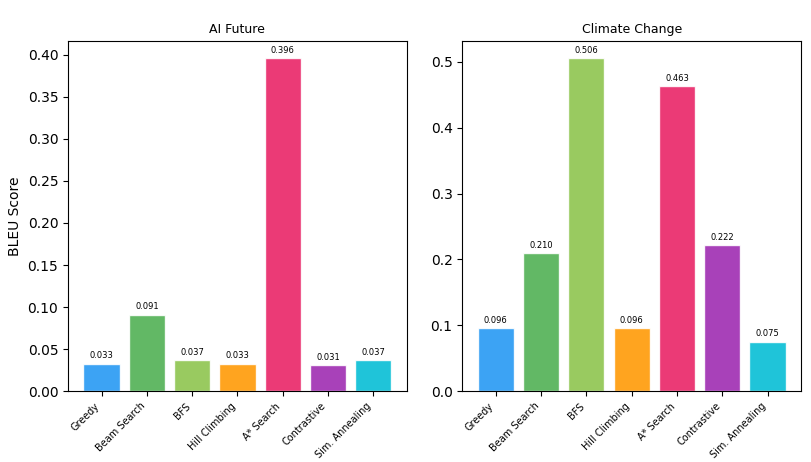
\includegraphics[width=0.8\linewidth]{Bleu/result_bleu_1.png}
	
	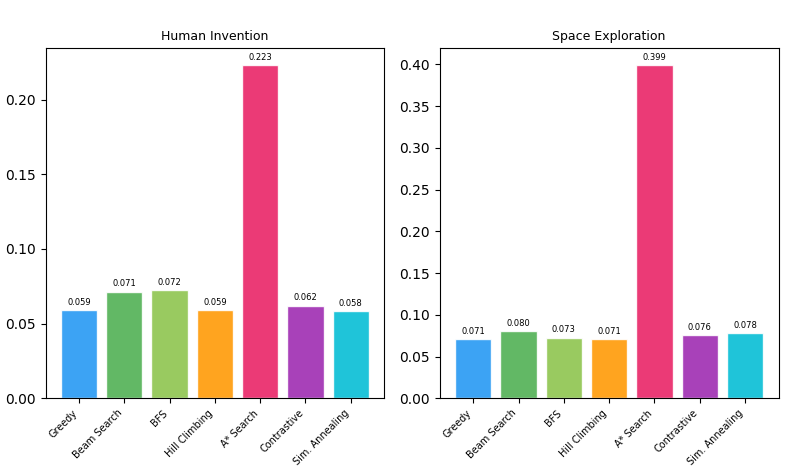
\includegraphics[width=0.8\linewidth]{Bleu/result_bleu_2.png}
	
	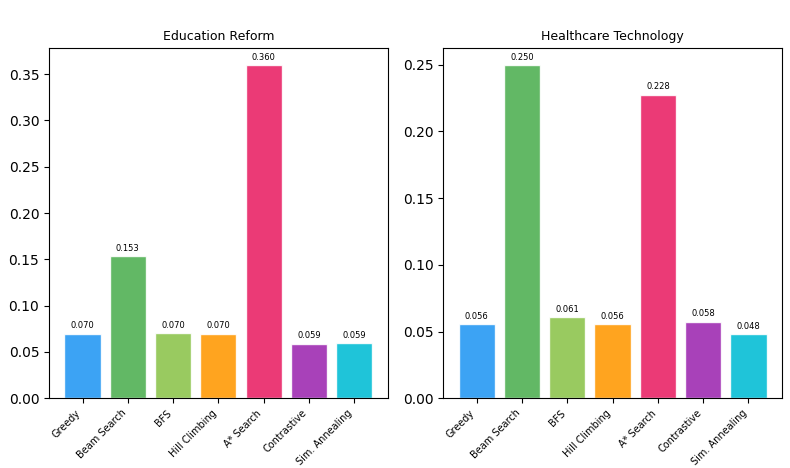
\includegraphics[width=0.8\linewidth]{Bleu/result_bleu_3.png}
	
	\caption{BLEU scores across all seven algorithms and six prompts.}
	\label{fig:bleu_all}
\end{figure}
	

\begin{table}[H]
	\centering
	\caption{Average BLEU scores across all six prompts}
	\label{tab:bleu_boxed}
	\small
	\setlength{\tabcolsep}{4pt}
	\begin{tabularx}{\linewidth}{|X|c|c|c|c|c|c|c|c|}
		\hline
		\textbf{Algorithm} & \textbf{P1} & \textbf{P2} & \textbf{P3} & \textbf{P4} & \textbf{P5} & \textbf{P6} & \textbf{Avg.} & \textbf{Rank} \\ \hline
		Greedy          & 0.033 & 0.096 & 0.059 & 0.071 & 0.070 & 0.056 & 0.064 & 5th \\ \hline
		Beam Search     & 0.091 & 0.210 & 0.071 & 0.080 & 0.153 & 0.250 & 0.143 & 2nd \\ \hline
		BFS             & 0.037 & 0.506 & 0.073 & 0.073 & 0.070 & 0.061 & 0.136 & 3rd \\ \hline
		Hill Climbing   & 0.033 & 0.096 & 0.059 & 0.071 & 0.070 & 0.056 & 0.064 & 5th \\ \hline
		A$^*$ Search    & \textbf{0.396} & \textbf{0.463} & \textbf{0.223} & \textbf{0.399} & \textbf{0.360} & \textbf{0.228} & \textbf{0.345} & \textbf{1st} \\ \hline
		Contrastive     & 0.031 & 0.222 & 0.062 & 0.076 & 0.059 & 0.058 & 0.085 & 4th \\ \hline
		Sim.\ Annealing & 0.034 & 0.071 & 0.061 & 0.076 & 0.058 & 0.045 & 0.058 & 7th \\ \hline
	\end{tabularx}
\end{table}

	\paragraph{A$^*$ dominates, but output length is the main driver.}
	A$^*$'s average BLEU of 0.345 is 2.4 times higher than Beam Search's 0.143. On P2 it reaches 0.463, a score that would be unusual for single-reference text generation. The mechanism behind this is not superior text quality but rather the interaction between very short output and short references; Section~\ref{sec:astar_paradox} unpacks this.
	
	\paragraph{Beam Search is a solid second.}
	Per-prompt scores range from 0.071 to 0.250, reflecting what five-candidate exploration buys you. P6 (Healthcare) scores highest because its reference uses high-frequency vocabulary that GPT-2 naturally assigns high probability.
	
	\paragraph{Hill Climbing matches Greedy exactly.}
	Identical BLEU scores across all six prompts, even with multi-token substitution, increased \texttt{top\_k=10}, and 3 random restarts. The null result is unambiguous.
	
	\paragraph{Simulated Annealing scores lowest.}
	Average BLEU of 0.058. Temperature sampling introduces tokens that are diverse but move away from the specific vocabulary of the reference sentences. Given the algorithm's design, this is not surprising.
	
	\begin{insightbox}{Cross-prompt BLEU pattern}
		The ranking (A$^*$ $\gg$ Beam $>$ BFS $>$ Contrastive $>$ Greedy $=$ Hill Climbing $>$ SA) holds across all six prompts, suggesting these are structural properties of the algorithms rather than prompt-specific artifacts.
	\end{insightbox}
	
	\subsection{BERTScore Analysis}
	\label{sec:bert}
	
	
\begin{figure}[H]
	\centering
	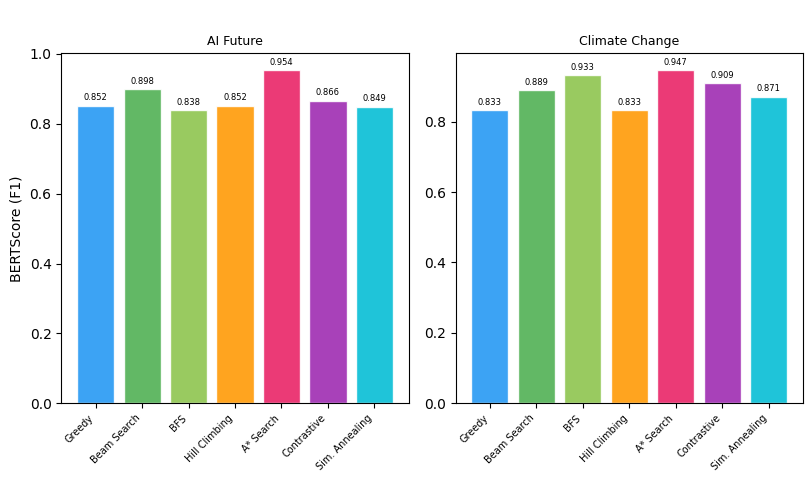
\includegraphics[width=0.8\linewidth]{Bert/bert_1.png}
	
	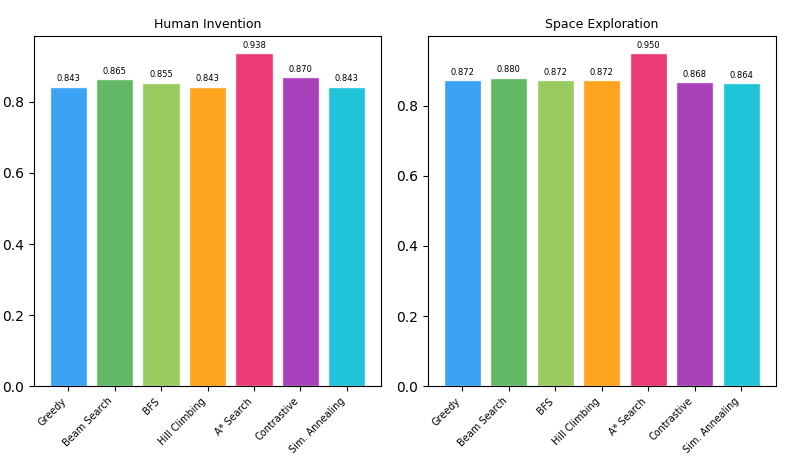
\includegraphics[width=0.8\linewidth]{Bert/bert_2.png}
	
	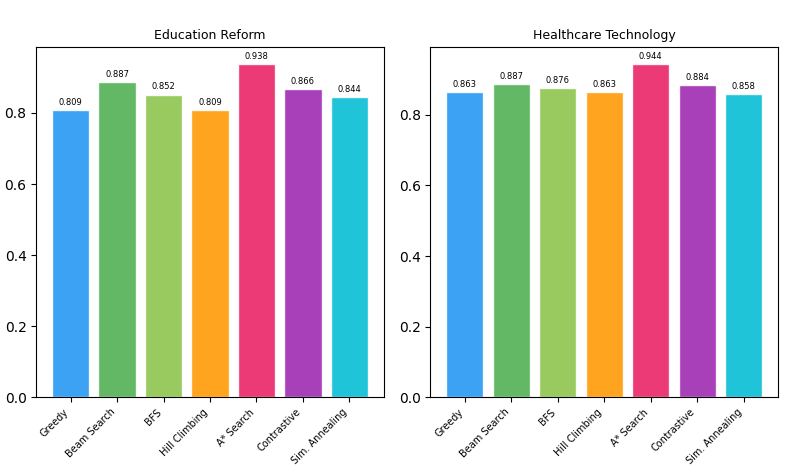
\includegraphics[width=0.8\linewidth]{Bert/bert_3.png}
	
	\caption{BERTScore (F1) across all seven algorithms and six prompts.}
	\label{fig:bert_all}
\end{figure}

	

\begin{table}[H]
	\centering
	\caption{Average BERTScore (F1) across all six prompts}
	\label{tab:bert_boxed}
	\small
	\setlength{\tabcolsep}{4pt}
	\begin{tabularx}{\linewidth}{|X|c|c|c|c|c|c|c|c|}
		\hline
		\textbf{Algorithm} & \textbf{P1} & \textbf{P2} & \textbf{P3} & \textbf{P4} & \textbf{P5} & \textbf{P6} & \textbf{Avg.} & \textbf{Rank} \\ \hline
		Greedy          & 0.852 & 0.833 & 0.843 & 0.872 & 0.809 & 0.863 & 0.845 & 6th \\ \hline
		Beam Search     & 0.898 & 0.889 & 0.865 & 0.880 & 0.887 & 0.887 & 0.884 & 2nd \\ \hline
		BFS             & 0.838 & 0.933 & 0.855 & 0.872 & 0.852 & 0.876 & 0.871 & 4th \\ \hline
		Hill Climbing   & 0.852 & 0.833 & 0.843 & 0.872 & 0.809 & 0.863 & 0.845 & 6th \\ \hline
		A$^*$ Search    & \textbf{0.954} & \textbf{0.947} & \textbf{0.938} & \textbf{0.950} & \textbf{0.938} & \textbf{0.944} & \textbf{0.945} & \textbf{1st} \\ \hline
		Contrastive     & 0.866 & 0.909 & 0.870 & 0.868 & 0.866 & 0.885 & 0.877 & 3rd \\ \hline
		Sim.\ Annealing & 0.853 & 0.848 & 0.843 & 0.851 & 0.841 & 0.860 & 0.849 & 5th \\ \hline
	\end{tabularx}
\end{table}
	
	\paragraph{A$^*$ leads by 0.061 over second place.}
	BERTScores of 0.938--0.954 indicate that A$^*$'s very short outputs are not just lexically similar to the references but semantically aligned at the embedding level. The core content words in each reference appear to be captured well in A$^*$'s compact, high-confidence output.
	
	\paragraph{Beam Search and Contrastive Search are close.}
	The difference is 0.007 (0.884 vs.\ 0.877). These two algorithms produce semantically similar output quality on these prompts.
	
	\paragraph{Greedy and Hill Climbing are again tied.}
	Both score 0.845. Hill Climbing's refinement procedure produces no measurable semantic improvement over its Greedy seed, confirming the null result from the BLEU analysis.
	
	\subsection{ROUGE-1 Score Analysis}
	\label{sec:rouge}
	
\begin{figure}[H]
	\centering
	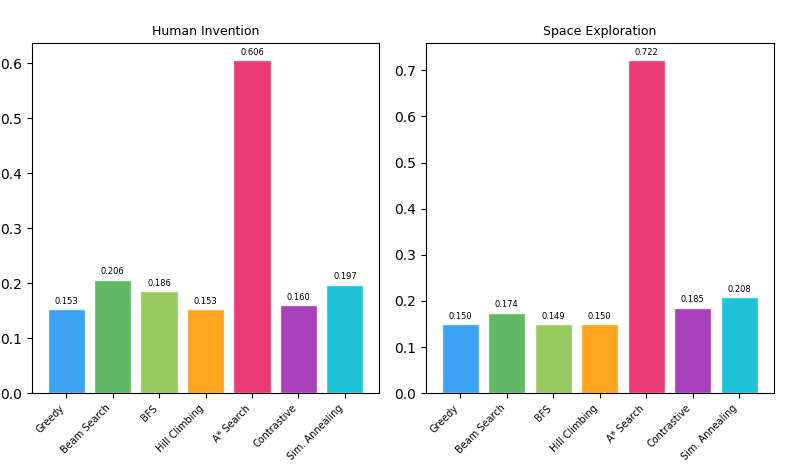
\includegraphics[width=0.8\linewidth]{Rouge/rouge_1.png}
	
	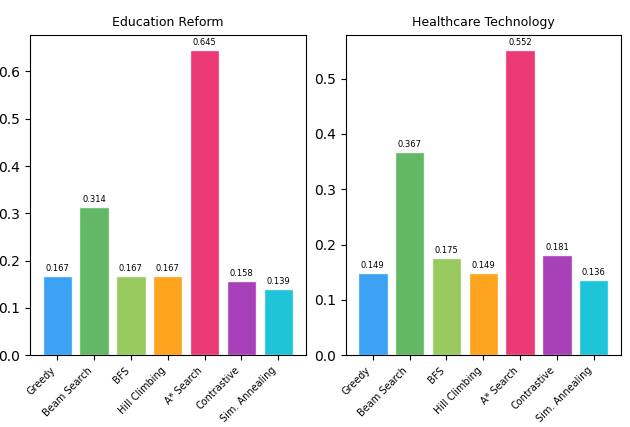
\includegraphics[width=0.8\linewidth]{Rouge/rouge_2.png}
	
	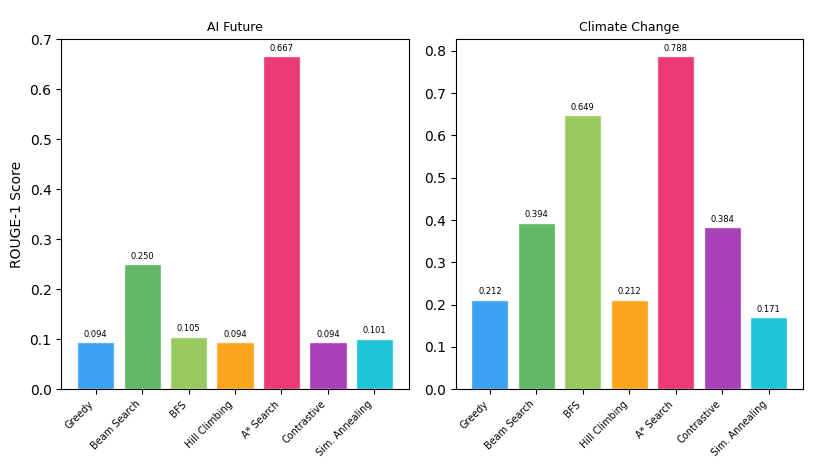
\includegraphics[width=0.8\linewidth]{Rouge/rouge_3.png}
	
	\caption{ROUGE-1 scores across all seven algorithms and six prompts.}
	\label{fig:rouge_all}
\end{figure}
	

\begin{table}[H]
	\centering
	\caption{Average ROUGE-1 scores across all six prompts}
	\label{tab:rouge_boxed}
	\small
	\setlength{\tabcolsep}{4pt}
	\begin{tabularx}{\linewidth}{|X|c|c|c|c|c|c|c|c|}
		\hline
		\textbf{Algorithm} & \textbf{P1} & \textbf{P2} & \textbf{P3} & \textbf{P4} & \textbf{P5} & \textbf{P6} & \textbf{Avg.} & \textbf{Rank} \\ \hline
		Greedy          & 0.095 & 0.212 & 0.153 & 0.150 & 0.167 & 0.149 & 0.154 & 5th \\ \hline
		Beam Search     & 0.250 & 0.394 & 0.207 & 0.175 & 0.314 & 0.367 & 0.284 & 2nd \\ \hline
		BFS             & 0.105 & 0.649 & 0.186 & 0.149 & 0.167 & 0.175 & 0.238 & 3rd \\ \hline
		Hill Climbing   & 0.095 & 0.212 & 0.153 & 0.150 & 0.167 & 0.149 & 0.154 & 5th \\ \hline
		A$^*$ Search    & \textbf{0.667} & \textbf{0.788} & \textbf{0.606} & \textbf{0.722} & \textbf{0.645} & \textbf{0.552} & \textbf{0.663} & \textbf{1st} \\ \hline
		Contrastive     & 0.094 & 0.384 & 0.161 & 0.185 & 0.158 & 0.181 & 0.194 & 4th \\ \hline
		Sim.\ Annealing & 0.090 & 0.160 & 0.185 & 0.183 & 0.127 & 0.110 & 0.142 & 7th \\ \hline
	\end{tabularx}
\end{table}

	\paragraph{A$^*$ achieves high recall from outputs under 15 words.}
	On P4 (Space Exploration), A$^*$'s 13-word output covers 72.2\% of the reference vocabulary. A$^*$'s priority queue converges on the highest-confidence tokens in GPT-2's distribution, and for factual prompts like these, those tokens tend to be the same semantically central words that appear in the reference.
	
	\paragraph{Beam Search holds second with a clear margin over BFS.}
	Per-prompt ROUGE scores range from 0.175 to 0.394, reflecting consistent vocabulary coverage. BFS ranks third (0.238), occasionally outperforming Beam Search on individual prompts (P2: ROUGE 0.649).
	
	\paragraph{Hill Climbing and Greedy tie across all six prompts.}
	Six prompts, six identical scores. The null result is now confirmed across a diverse prompt set.
	
	\subsection{Execution Time Analysis}
	\label{sec:time}
	
	\begin{figure}[H]
		\centering
		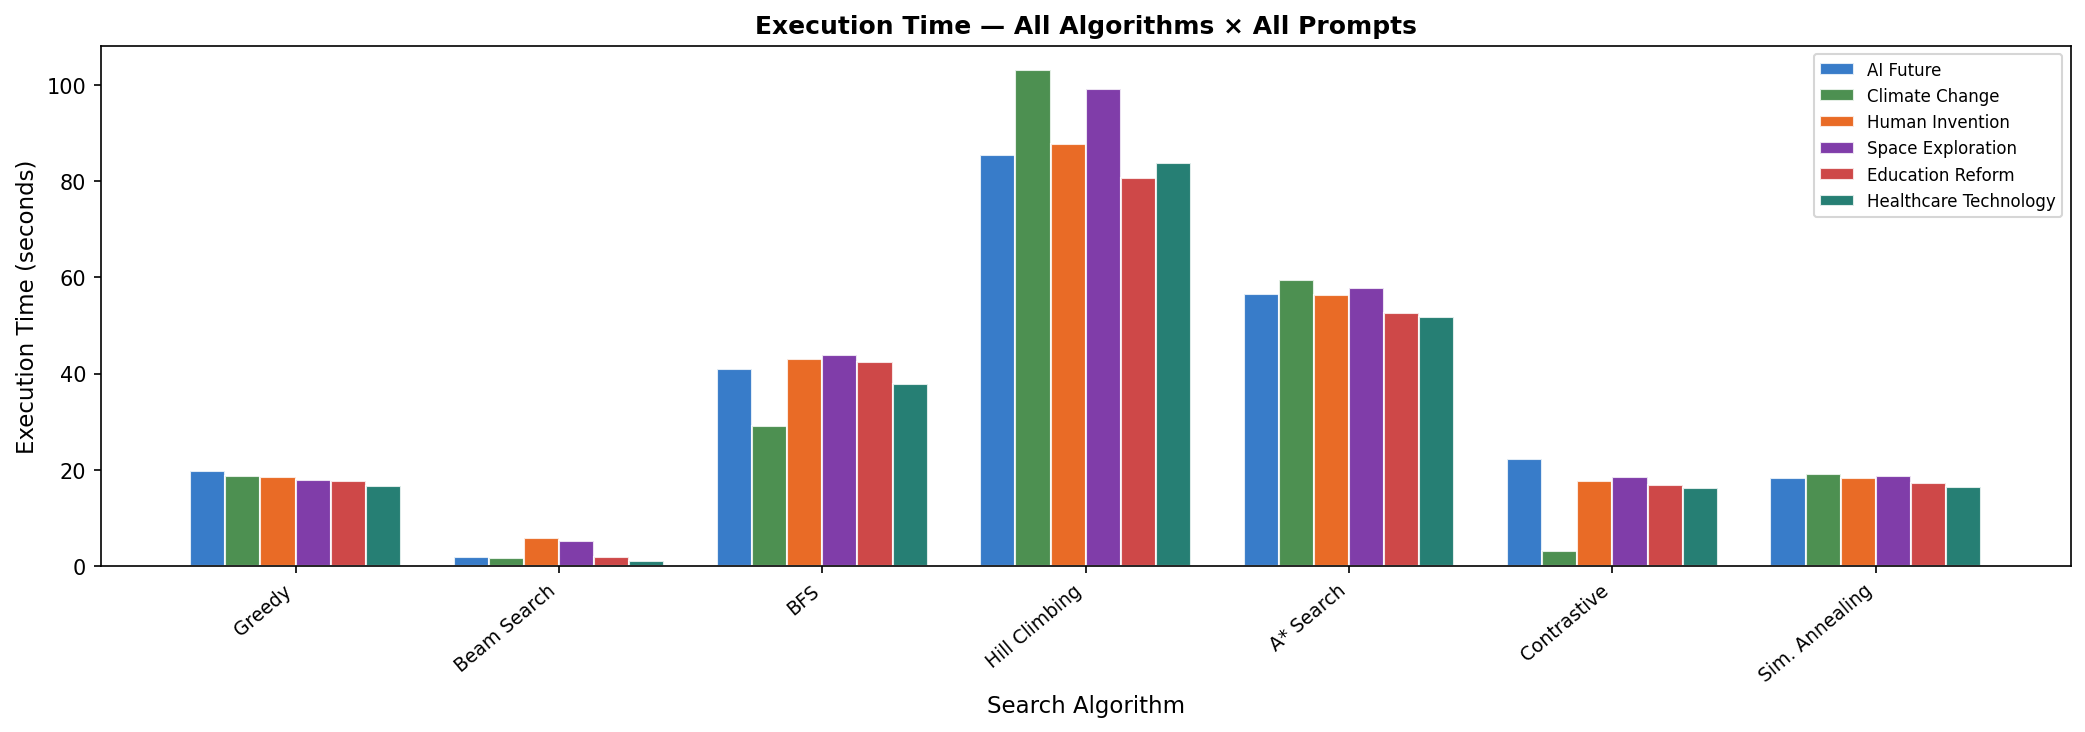
\includegraphics[width=\linewidth]{result_time.png}
		\caption{Execution time (seconds) across all seven algorithms and six prompts.}
		\label{fig:time_all}
	\end{figure}
	
\begin{table}[H]
	\centering
	\caption{Average execution time (seconds) across all six prompts}
	\label{tab:time_boxed}
	\small
	\setlength{\tabcolsep}{4pt}
	\begin{tabularx}{\linewidth}{|X|c|c|}
		\hline
		\textbf{Algorithm} & \textbf{Avg. Time (s)} & \textbf{Rank} \\ \hline
		Greedy          & $\sim$19   & 3rd \\ \hline
		Beam Search     & \textbf{$\sim$3} & \textbf{1st} \\ \hline
		BFS             & $\sim$38   & 5th \\ \hline
		Hill Climbing   & $\sim$111  & 7th \\ \hline
		A$^*$ Search    & $\sim$71   & 6th \\ \hline
		Contrastive     & $\sim$19   & 3rd \\ \hline
		Sim.\ Annealing & $\sim$27   & 4th \\ \hline
	\end{tabularx}
\end{table}
	
	\paragraph{Beam Search is the fastest at $\sim$3 seconds on average.}
	This seems counterintuitive: five beams finishing faster than a single greedy pass. The explanation is implementation, not theory. HuggingFace's \texttt{generate()} function is compiled and batched, processing all five beams in parallel via vectorised tensor operations. Greedy Search, by contrast, uses an explicit Python loop that calls model inference sequentially.
	
	\paragraph{Hill Climbing peaks at 200 seconds on P4 (Space Exploration).}
	On its own, that number is bad. In context, it is worse: Hill Climbing also delivers zero quality improvement over Greedy Search. The multi-token substitution and random restarts added in Version~3.0 increase computation time but do not escape the local optimum.
	
	\paragraph{A$^*$ at $\sim$71 seconds is explainable but expensive.}
	Even though A$^*$ terminates after 7--13 words, it explores many candidate extensions before committing to each output token. The cached heuristic in Version~3.0 reduced this from $\sim$114 seconds in Version~2.0, but the algorithm remains slow.
	
	\paragraph{Contrastive Search at $\sim$19 seconds matches Greedy's speed.}
	The cosine similarity calculations add modest overhead. This makes Contrastive Search the best practical alternative when diversity matters.
	
	\subsection{Generated Text Length Analysis}
	\label{sec:length}
	
	\begin{figure}[H]
		\centering
		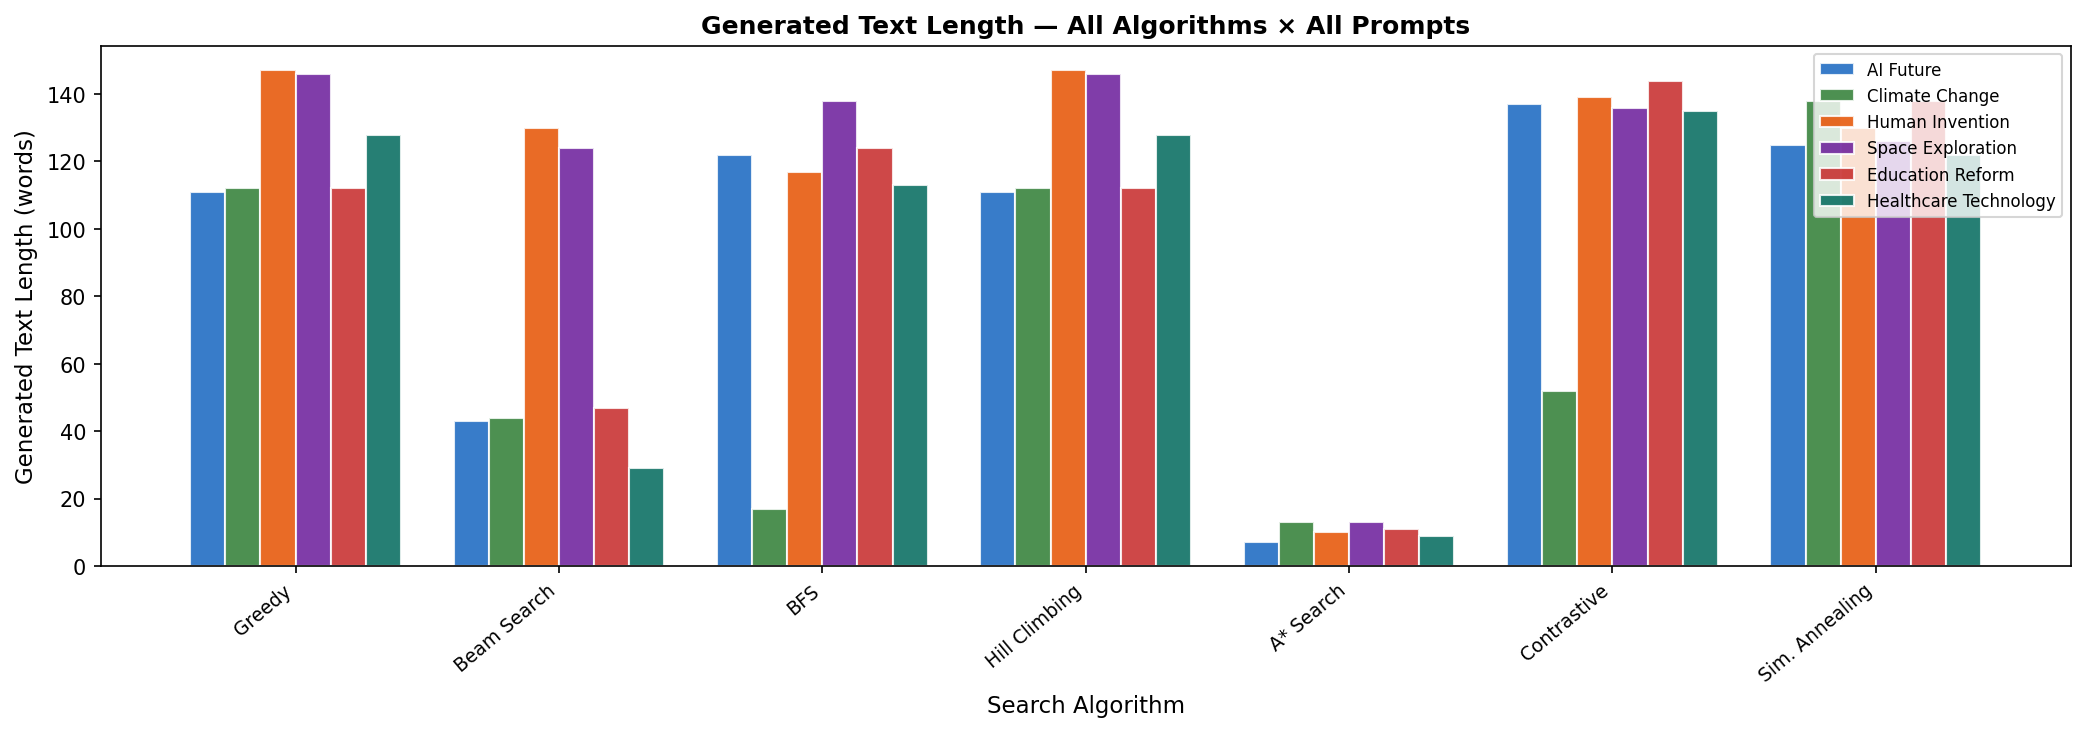
\includegraphics[width=\linewidth]{result_length.png}
		\caption{Generated text length (words) across all seven algorithms and six prompts.}
		\label{fig:length_all}
	\end{figure}
	
\begin{table}[H]
	\centering
	\caption{Average generated text length (words) across all six prompts}
	\label{tab:length_boxed}
	\small
	\setlength{\tabcolsep}{3pt}
	\begin{tabularx}{\linewidth}{|X|c|c|}
		\hline
		\textbf{Algorithm} & \textbf{Avg. Words} & \textbf{Character} \\ \hline
		Greedy          & 126 & Long \\ \hline
		Beam Search     & 70  & Concise \\ \hline
		BFS             & 105 & Medium-long \\ \hline
		Hill Climbing   & 126 & Long (= Greedy) \\ \hline
		A$^*$ Search    & \textbf{11} & Very short \\ \hline
		Contrastive     & 124 & Long \\ \hline
		Sim.\ Annealing & 135 & Longest \\ \hline
	\end{tabularx}
\end{table}
	
	\paragraph{A$^*$'s improved heuristic helped, but did not solve the problem.}
	Version~1.0 generated 7 words for its single prompt. Version~3.0 generates 7--13 words across six prompts. Despite the increased $\alpha = 0.8$ and minimum-length penalty, 7--13 words remain far below the 150-token limit. The heuristic still decreases as the sequence grows, because the numerator (sum of negative log-probabilities) shrinks faster than the denominator ($T^{0.8}$) increases. A stronger normalisation or an explicit length bonus would be needed to fix this properly.
	
	\paragraph{Hill Climbing lengths equal Greedy lengths exactly.}
	In-place substitution cannot change sequence length. Both algorithms produce 126 words on average.
	
	\paragraph{Simulated Annealing generates the longest outputs.}
	At high temperature, the token distribution is nearly uniform, so low-probability tokens (including EOS) are rare early in generation. By the time temperature cools enough for EOS to become likely, the sequence is already long. Average: 135 words.
	
	\subsection{Average Scores and Cross-Prompt Consistency}
	\label{sec:avg}
	
	\begin{figure}[H]
		\centering
		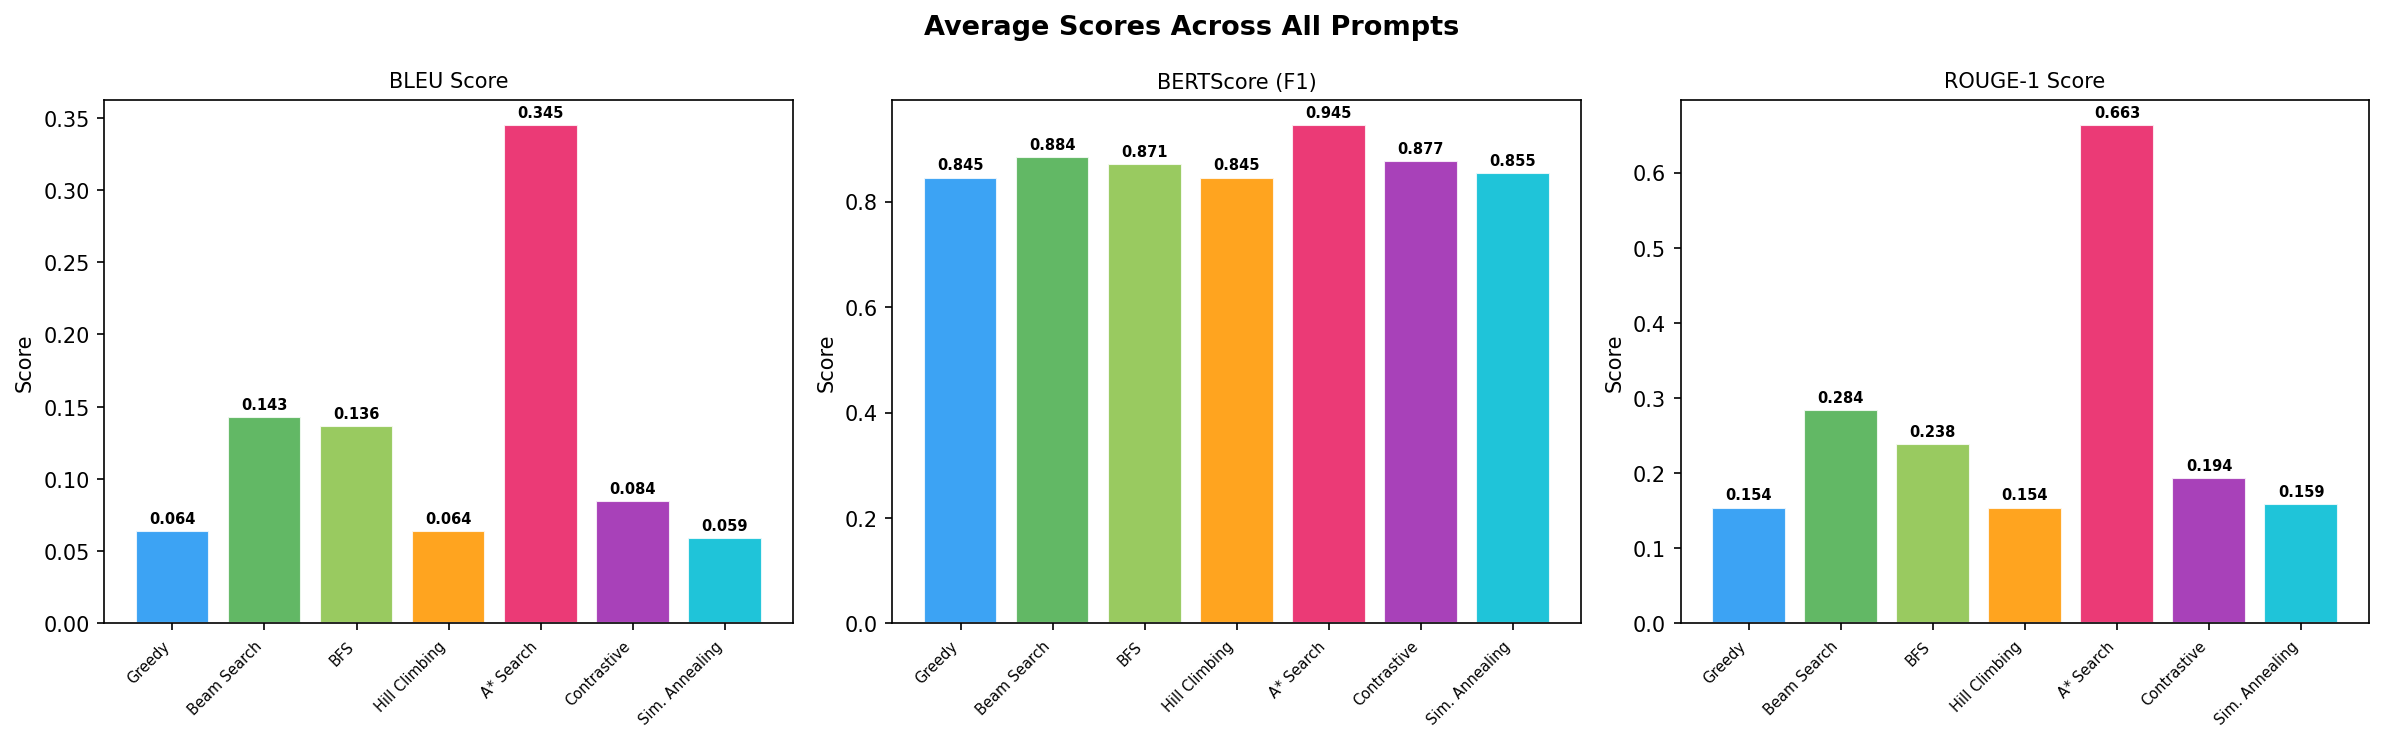
\includegraphics[width=\linewidth]{result_avg_summary.png}
		\caption{Average BLEU, BERTScore, and ROUGE-1 across all six prompts.}
		\label{fig:avg_summary}
	\end{figure}
	
	Figure~\ref{fig:avg_summary} shows the averaged results. Several patterns stand out.
	
	The ranking on all three quality metrics is consistent across all six prompts. A$^*$ leads every time. Beam Search is second on BLEU and ROUGE. Hill Climbing ties Greedy every time. Simulated Annealing sits at or near the bottom every time. This consistency across prompts with different vocabulary and domain characteristics means the differences reflect structural properties of the algorithms, not quirks of individual prompts.
	
	Execution time, by contrast, varies more across prompts. Hill Climbing on P4 takes 200 seconds while P1 takes 62 seconds, reflecting the prompt-dependent cost of the multi-position scanning in Phase~2.
	
	% =============================================================================
	\section{Discussion}
	\label{sec:discussion}
	% =============================================================================
	
	\subsection{The A* Paradox: Dominant Scores from 10-Word Outputs}
	\label{sec:astar_paradox}
	
	The most important result in this study needs an honest explanation, not celebration. A$^*$ Search scores highest on BLEU, BERTScore, and ROUGE-1. It also generates outputs of 7--13 words. These two facts are connected.
	
	Here is what happens. The reference sentences are 8--20 words. A$^*$'s priority queue consistently favours partial sequences that are short, high-confidence, and semantically central to the prompt. When a 7-word output is evaluated against a 12-word reference:
	
	\begin{itemize}[leftmargin=*]
		\item \textbf{BLEU precision} is high: most generated words appear in the reference. The brevity penalty is modest because the reference itself is short.
		\item \textbf{ROUGE-1 recall} is high: the generated words cover several of the reference's key unigrams.
		\item \textbf{BERTScore} is high: A$^*$'s confident, semantically central tokens map closely to the reference embeddings.
	\end{itemize}
	
	This is not a flaw in A$^*$, and it is not a flaw in the metrics. It is a real property of A$^*$'s behaviour that happens to interact favourably with these metrics on these prompts. The algorithm \emph{is} selecting the most semantically precise, highest-confidence tokens. The issue is that the global priority structure causes it to stop after producing a handful of them, before completing a full sentence.
	
	The practical implication matters: A$^*$'s metric dominance does not mean it would be the right choice in a real application. If a user asks a chatbot to finish a sentence and gets back 7 words, the response will feel incomplete regardless of its BLEU score. For applications that need full, informative continuations, Beam Search or Contrastive Search are better choices. A$^*$ in its current form fits applications that specifically want a short, high-confidence completion, like autocomplete suggestions or keyword extraction.
	
	\subsection{Hill Climbing: Why the Null Result Persists}
	\label{sec:hillclimb_discussion}
	
	Hill Climbing matched Greedy exactly on BLEU and ROUGE across all six prompts, even with multi-token substitution (\texttt{top\_k=10}), 5 iterations, and 3 random restarts. On BERTScore the scores are identical (0.845). This is a null result, and it has a clear explanation.
	
	The core issue is that Greedy Search produces a sequence that is already locally optimal with respect to the objective Hill Climbing uses. Each token in the Greedy output was chosen to maximise $P(t_i \mid p, t_1, \ldots, t_{i-1})$ at the time of generation. Phase~2 checks whether any substitution at the worst-scoring positions improves the \emph{average} log-probability across the whole sequence. For GPT-2 on these prompts, the answer turns out to be: almost never. The Greedy output sits at or very near a local optimum of Equation~\eqref{eq:hill_quality}.
	
	There is a second, structural reason. Hill Climbing optimises average log-probability, not n-gram overlap with the reference. Even if a substitution did improve average log-probability, it would only improve BLEU or ROUGE if the new token happened to match a reference token. The optimisation target and the evaluation criteria are not aligned.
	
	The practical conclusion is straightforward: this implementation of Hill Climbing should not be used as a decoding strategy. It costs up to 200 seconds and delivers nothing over Greedy.
	
	\subsection{Beam Search as the Production Default}
	\label{sec:beam_discussion}
	
	Beam Search ranks second on all three quality metrics, first on speed ($\sim$3 seconds), and produces outputs of practical length (29--130 words). It is the recommended default for most applications.
	
	Five-candidate exploration finds token combinations that single-path methods miss. On P6 (Healthcare), Beam Search achieves BLEU of 0.250 and ROUGE of 0.367, the highest among the algorithms that produce long output. The no-repeat-bigram constraint prevents the most obvious repetition patterns.
	
	The $\sim$3-second execution time warrants comment. Beam Search is faster than Greedy ($\sim$19 seconds) in these experiments because HuggingFace's batched \texttt{generate()} processes all five beams in parallel using vectorised tensor operations, while Greedy uses an explicit Python loop.
	
	\subsection{BFS: A Classical Search Baseline}
	\label{sec:bfs_discussion}
	
	BFS ranks third on BLEU (0.136) and ROUGE (0.238), occasionally outperforming Beam Search on individual prompts (P2: BLEU 0.506, ROUGE 0.649). However, at $\sim$38 seconds average it is 13 times slower than Beam Search. BFS also falls into the same repetition trap as Greedy during its greedy extension phase: P1 repeats the Musk/Brin sentence 7 times, P3 repeats ``The automobile is the most revolutionary invention'' 10 times.
	
	The P2 result is particularly interesting. BFS produced only 17 words and hit EOS early, but those 17 words happened to overlap well with the reference, yielding the highest single-prompt BLEU score in the entire study (0.506). This is another instance of the metric-length interaction that also drives A$^*$'s dominance.
	
	\subsection{Contrastive Search: A Practical Alternative}
	\label{sec:contrastive_discussion}
	
	Contrastive Search ranks third on BERTScore (0.877) and fourth on BLEU (0.085) and ROUGE (0.194), and runs in about $\sim$19 seconds. For applications where output diversity and avoidance of semantic repetition matter (creative writing, dialogue systems, or any scenario where the same prompt is used repeatedly), Contrastive Search is a better fit than Beam Search.
	
	The generated outputs confirm this: across all six prompts, Contrastive Search produces the most topically varied and non-repetitive long-form text. None of its outputs contain the looping patterns seen in Greedy, Hill Climbing, BFS, or even Simulated Annealing.
	
	\subsection{Simulated Annealing: Creative but Imprecise}
	\label{sec:sa_discussion}
	
	Simulated Annealing generates the longest outputs (135 words on average) and scores lowest or near-lowest on all quality metrics: BLEU 0.058, ROUGE 0.142, BERTScore 0.849. This is expected. High initial temperature lets the algorithm select improbable tokens that diverge from the reference vocabulary.
	
	The right way to interpret this is that Simulated Annealing is optimising for something different from what these metrics measure. It is not trying to match a reference sentence; it is exploring the probability space broadly at the start and narrowing gradually. For tasks where novelty matters more than reference alignment (storytelling, brainstorming, diverse data generation), its practical value may be higher than these scores suggest.
	
	One limitation deserves emphasis: these results come from a single run. Simulated Annealing samples stochastically, so its quality varies between runs. Ten or twenty runs averaged together would give a more statistically reliable picture.
	
	\subsection{Cross-Algorithm Comparison: A Unified View}
	
	Table~\ref{tab:comparison_boxed} summarises the seven algorithms across all dimensions evaluated.
	
\begin{table}[H]
	\centering
	\caption{Comprehensive cross-algorithm comparison}
	\label{tab:comparison_boxed}
	\footnotesize
	\setlength{\tabcolsep}{3pt}
	\begin{tabularx}{\linewidth}{|X|c|c|c|c|c|X|}
		\hline
		\textbf{Algorithm} & \textbf{Quality} & \textbf{Speed} & \textbf{Length} & \textbf{Det.} & \textbf{Verdict} & \textbf{Best Application} \\ \hline
		Greedy          & Low    & Medium & Long    & Yes & Avoid    & Baseline comparison \\ \hline
		Beam Search     & High   & Fast   & Medium  & Yes & Recommend & Production NLP \\ \hline
		BFS             & Medium & Slow   & Long    & Yes & Baseline  & Classical search baseline \\ \hline
		Hill Climbing   & Low    & Slow   & Long    & Yes & Avoid    & None (null result) \\ \hline
		A$^*$ Search    & Highest& Slow   & V. Short& Yes & Special.  & Short-answer precision \\ \hline
		Contrastive     & High   & Medium & Long    & Yes & Recommend & Diverse output \\ \hline
		Sim.\ Annealing & Low    & Medium & Longest & No  & Creative  & Creative generation \\ \hline
	\end{tabularx}
\end{table}
	
	% =============================================================================
	\section{Threats to Validity}
	\label{sec:threats}
	% =============================================================================
	
	No experiment is flawless. This section identifies the main threats to the conclusions.
	
	\subsection{Internal Validity}
	
	\paragraph{Single-run results for Simulated Annealing.}
	SA is stochastic, and a single run may not represent the distribution of its outputs. Future work should run at least 10 seeds and report mean and variance.
	
	\paragraph{Hill Climbing parameter sensitivity.}
	\texttt{top\_k} = 10, \texttt{max\_iter} = 5, and \texttt{num\_restarts} = 3 were chosen to improve over Version~2.0's settings (\texttt{top\_k} = 5, \texttt{max\_iter} = 3, no restarts), but still produced a null result. With \texttt{top\_k} = 50 or \texttt{max\_iter} = 20, Phase~2 might find substitutions that escape the local optimum. The null result reported here is specific to these parameter settings.
	
	\paragraph{A$^*$'s length penalty parameter.}
	$\alpha = 0.8$ was increased from 0.7 in Version~2.0 and augmented with a minimum-length penalty of 20 tokens, but A$^*$ still produces outputs of only 7--13 words. A different value (e.g., $\alpha = 0.95$ or a multiplicative length bonus) might produce longer outputs. This parameter was not exhaustively tuned.
	
	\subsection{External Validity}
	
	\paragraph{Six prompts across six domains.}
	Six prompts provide more evidence than the single prompt in Version~1.0, but they cannot represent the full range of text generation tasks. Prompts with longer references, domain-specific vocabulary, or multi-sentence structure might produce different rankings.
	
	\paragraph{GPT-2 is not a current model.}
	Modern models like GPT-4, LLaMA-3, and Mistral produce fundamentally different probability distributions. The rankings observed here may not transfer to larger, more capable models where probability mass is distributed differently across the vocabulary.
	
	\paragraph{Single reference sentences.}
	All three metrics assume one correct continuation. In reality, many valid continuations exist. Algorithms that produce alternative but high-quality continuations (Simulated Annealing and Contrastive Search deliberately seek these) get penalised under this evaluation setup.
	
	\subsection{Construct Validity}
	
	\paragraph{Metric-length interaction.}
	As discussed in Sections~\ref{sec:results} and~\ref{sec:discussion}, A$^*$'s metric dominance is partly a function of its short outputs rather than purely superior generation quality. Any future study comparing algorithms with very different output length profiles should account for this interaction, ideally by normalising for length or by adding length-controlled evaluations.
	
	\paragraph{Execution time on a single machine.}
	Timing measurements were taken on one machine with no load control. Background processes, CPU vs.\ GPU differences, and caching effects all introduce noise.
	
	% =============================================================================
	\section{Conclusion and Future Work}
	\label{sec:conclusion}
	% =============================================================================
	
	\subsection{Summary of Findings}
	
	This study compared seven heuristic search decoding algorithms for GPT-2 text generation across six prompts, evaluating BLEU, BERTScore, ROUGE-1, execution time, and output length. The main findings:
	
	\begin{enumerate}[leftmargin=*]
		\item \textbf{A$^*$ Search scores highest on all three quality metrics} (BLEU 0.345, BERTScore 0.945, ROUGE 0.663 on average). The result is real but requires careful interpretation: A$^*$'s short outputs (7--13 words) interact favourably with the evaluation metrics against short reference sentences. It is best suited for applications requiring brief, high-precision completions.
		
		\item \textbf{The improved A$^*$ heuristic} (cached computation, $\alpha = 0.8$, minimum-length penalty) reduced GPT-2 forward passes by roughly half compared to Version~2.0, but still did not fully eliminate the short-output bias. Output lengths remain 7--13 words.
		
		\item \textbf{Beam Search is the best practical algorithm}: second on all quality metrics, fastest execution ($\sim$3 seconds average), and produces complete, coherent outputs of 29--130 words. It is the recommended default.
		
		\item \textbf{BFS provides a useful classical baseline}: it ranks third on BLEU (0.136) and ROUGE (0.238), occasionally outperforming Beam Search on individual prompts (P2: BLEU 0.506), but at $\sim$38 seconds average it is 13 times slower than Beam Search.
		
		\item \textbf{Hill Climbing yields a null result even with improvements}: despite multi-token substitution, increased \texttt{top\_k=10}, 5 iterations, and 3 random restarts, it still produces identical BLEU and ROUGE to Greedy Search across all six prompts, while being 6 times slower.
		
		\item \textbf{Contrastive Search} produces the most topically diverse and non-repetitive long-form output, ranking third on BERTScore (0.877) with execution time comparable to Greedy.
		
		\item \textbf{Simulated Annealing} generates the longest outputs (135 words average) but scores lowest on all quality metrics. Its stochastic nature produces erratic content, particularly at high initial temperature.
	\end{enumerate}
	
	\subsection{Recommendations for Future Research}
	
	\paragraph{1. Improve the A$^*$ heuristic further.}
	The cached heuristic in Version~3.0 reduced GPT-2 calls by $\sim$50\%, and $\alpha = 0.8$ with a minimum-length penalty of 20 tokens was an improvement over $\alpha = 0.7$, but A$^*$ still produces only 7--13 words. An explicit length bonus such as $h(n) = \sum \log p / T^{\alpha} + \beta T$ could encourage longer outputs. Alternatively, a learned value function trained to predict reference similarity at full length would eliminate hand-crafted heuristic design entirely.
	
	\paragraph{2. Improve Hill Climbing beyond multi-token substitution.}
	Version~3.0's multi-token substitution, increased \texttt{top\_k=10}, and random restarts were insufficient to escape the local optima. Future work should test: (a) simultaneous substitution of the $k$ worst positions; (b) a substitution objective that directly targets BLEU or ROUGE rather than average log-probability; (c) larger values of \texttt{top\_k} (50+) and \texttt{max\_iter} (20+).
	
	\paragraph{3. Improve BFS with anti-repetition constraints.}
	BFS's greedy extension phase suffers from the same repetition as Greedy Search. Adding a no-repeat-bigram constraint (as Beam Search uses) to the greedy extension would likely improve BFS's output quality without affecting its BFS exploration phase.
	
	\paragraph{4. Expand and diversify the prompt set further.}
	Version~3.0 uses six prompts across six domains, up from one prompt in Version~1.0. Future work should test on an even larger set: longer prompts, multi-sentence prompts, domain-specific prompts (medical, legal, technical), and prompts where the expected continuation is ambiguous. The 150-token limit should also be increased to 200 or more tokens.
	
	\paragraph{5. Test on larger models.}
	GPT-2 (117M parameters) is small by current standards. Testing on GPT-2 Medium (345M), GPT-3, LLaMA-3, Mistral, or GPT-J would establish whether the algorithm rankings generalise to more capable models. The code already supports GPT-2 Medium by changing a single variable (\texttt{MODEL\_NAME}).
	
	\paragraph{6. Human evaluation study.}
	Automatic metrics cannot capture fluency, coherence, engagement, or practical usefulness. A human evaluation study asking raters to rank outputs from all seven algorithms per prompt would complement the automatic results. Given that A$^*$ produces outputs under 13 words while Beam Search produces 29--130 words, human raters would almost certainly rank them very differently from the metrics.
	
	% =============================================================================
	% Appendix
	% =============================================================================
	\newpage
	\appendix
	
	\section{Generated Outputs}
	\label{app:outputs}
	
	 These are the complete, unedited outputs from the Version~3.0 experimental runs (7 algorithms, 6 prompts). Full raw text is also available in the GitHub repository at \texttt{all\_outputs.txt}.
	
\setlength{\fboxsep}{6pt}

\subsection*{Prompt P1: ``The future of artificial intelligence is''}

\noindent\fbox{\begin{minipage}{\dimexpr\linewidth-2\fboxsep-2\fboxrule\relax}
\textbf{Greedy / Hill Climbing:} The future of artificial intelligence is uncertain. ``We're not sure what the future will look like,'' said Dr.\ Michael S.\ Schoenfeld, a professor of computer science at the University of California, Berkeley. ``But we're not sure what the future will look like for artificial intelligence.'' \textit{[entire block repeats; 111 words]}
\end{minipage}}

\vspace{3pt}
\noindent\fbox{\begin{minipage}{\dimexpr\linewidth-2\fboxsep-2\fboxrule\relax}
\textbf{Beam Search:} The future of artificial intelligence is in the hands of the next generation of scientists and engineers. ``It's a very exciting time to be a part of it,'' he said. ``I think it's going to take a lot of work to get there.'' \textit{[43 words]}
\end{minipage}}

\vspace{3pt}
\noindent\fbox{\begin{minipage}{\dimexpr\linewidth-2\fboxsep-2\fboxrule\relax}
\textbf{BFS:} The future of artificial intelligence is in the hands of people like Elon Musk and Sergey Brin. \textit{[sentence repeats 7 times due to greedy extension; 122 words]}
\end{minipage}}

\vspace{3pt}
\noindent\fbox{\begin{minipage}{\dimexpr\linewidth-2\fboxsep-2\fboxrule\relax}
\textbf{A$^*$ Search:} The future of artificial intelligence is uncertain \textit{[7 words]}
\end{minipage}}

\vspace{3pt}
\noindent\fbox{\begin{minipage}{\dimexpr\linewidth-2\fboxsep-2\fboxrule\relax}
\textbf{Contrastive:} The future of artificial intelligence is uncertain. But there are signs that AI could soon surpass human intelligence in terms of its ability to solve complex problems and perhaps even improve upon existing ones. A recent paper published online today suggests artificial intelligence may be able to help us understand how people live their lives better than we do now\ldots\ \textit{[137 words; no repetition]}
\end{minipage}}

\vspace{3pt}
\noindent\fbox{\begin{minipage}{\dimexpr\linewidth-2\fboxsep-2\fboxrule\relax}
\textbf{Sim.\ Annealing:} The future of artificial intelligence is sluggish'' ReutersImage start-up Asher Schwartz. The Swedish researchers said the new technology could help humans learn to be more self-aware\ldots\ \textit{[erratic; 118 words]}
\end{minipage}}

%─────────────────────────────────────────────────────────────────
\subsection*{Prompt P2: ``Climate change is one of the most pressing challenges facing humanity because''}

\noindent\fbox{\begin{minipage}{\dimexpr\linewidth-2\fboxsep-2\fboxrule\relax}
\textbf{Greedy / Hill Climbing:} Climate change is one of the most pressing challenges facing humanity because it is the most complex and complex problem in the world. The world is changing rapidly\ldots\ \textit{[``The world is changing rapidly'' repeats 16 times; 112 words]}
\end{minipage}}

\vspace{3pt}
\noindent\fbox{\begin{minipage}{\dimexpr\linewidth-2\fboxsep-2\fboxrule\relax}
\textbf{Beam Search:} Climate change is one of the most pressing challenges facing humanity because of climate change. ``We need to make sure that we have the resources to deal with it,'' he said. ``It's not going to happen overnight, but it's a long way from now.'' \textit{[44 words]}
\end{minipage}}

\vspace{3pt}
\noindent\fbox{\begin{minipage}{\dimexpr\linewidth-2\fboxsep-2\fboxrule\relax}
\textbf{BFS:} Climate change is one of the most pressing challenges facing humanity because of climate change,'' he said. \textit{[17 words; BFS hit EOS early; highest BLEU on this prompt at 0.506]}
\end{minipage}}

\vspace{3pt}
\noindent\fbox{\begin{minipage}{\dimexpr\linewidth-2\fboxsep-2\fboxrule\relax}
\textbf{A$^*$ Search:} Climate change is one of the most pressing challenges facing humanity because it \textit{[13 words]}
\end{minipage}}

\vspace{3pt}
\noindent\fbox{\begin{minipage}{\dimexpr\linewidth-2\fboxsep-2\fboxrule\relax}
\textbf{Contrastive:} Climate change is one of the most pressing challenges facing humanity because it affects millions of people around the world. But climate change is also one of humanity's greatest challenges because it impacts so many different parts of us and our lives every day. This article originally appeared on VICE News UK \textit{[52 words]}
\end{minipage}}

\vspace{3pt}
\noindent\fbox{\begin{minipage}{\dimexpr\linewidth-2\fboxsep-2\fboxrule\relax}
\textbf{Sim.\ Annealing:} Climate change is one of the most pressing challenges facing humanity because policy makers complicate increasing certainty that feeding food to consumers and businesses is the only way to address climate change\ldots\ \textit{[141 words]}
\end{minipage}}

%─────────────────────────────────────────────────────────────────
\subsection*{Prompt P3: ``The most revolutionary invention in human history has been''}

\noindent\fbox{\begin{minipage}{\dimexpr\linewidth-2\fboxsep-2\fboxrule\relax}
\textbf{Greedy / Hill Climbing:} The most revolutionary invention in human history has been the invention of the telephone. The telephone was invented by the French in 1848. It was a telephone that could be used to communicate with any person\ldots\ \textit{[repeats 9 times; 147 words]}
\end{minipage}}

\vspace{3pt}
\noindent\fbox{\begin{minipage}{\dimexpr\linewidth-2\fboxsep-2\fboxrule\relax}
\textbf{Beam Search:} The most revolutionary invention in human history has been the invention of the atomic bomb. The bomb was designed to destroy Hiroshima and Nagasaki, the two largest cities in Japan\ldots\ \textit{[130 words]}
\end{minipage}}

\vspace{3pt}
\noindent\fbox{\begin{minipage}{\dimexpr\linewidth-2\fboxsep-2\fboxrule\relax}
\textbf{BFS:} The most revolutionary invention in human history has been the invention of the automobile. The automobile is the most revolutionary invention in human history\ldots\ \textit{[repeats 10 times; 117 words]}
\end{minipage}}

\vspace{3pt}
\noindent\fbox{\begin{minipage}{\dimexpr\linewidth-2\fboxsep-2\fboxrule\relax}
\textbf{A$^*$ Search:} The most revolutionary invention in human history has been the \textit{[10 words]}
\end{minipage}}

\vspace{3pt}
\noindent\fbox{\begin{minipage}{\dimexpr\linewidth-2\fboxsep-2\fboxrule\relax}
\textbf{Contrastive:} The most revolutionary invention in human history has been the invention of radio waves. It was first proposed by Albert Einstein in 1887 when he discovered how electromagnetic fields can be generated using an oscillator called ``electrode magnetism''\ldots\ \textit{[139 words; diverse but factually incorrect]}
\end{minipage}}

\vspace{3pt}
\noindent\fbox{\begin{minipage}{\dimexpr\linewidth-2\fboxsep-2\fboxrule\relax}
\textbf{Sim.\ Annealing:} The most revolutionary invention in human history has been fans circular idea smashing AppleMouse. Avella has revealed that they have partnered with the company to develop a new version of the mouse\ldots\ \textit{[erratic; 139 words]}
\end{minipage}}

%─────────────────────────────────────────────────────────────────
\subsection*{Prompt P4: ``The primary goal of space exploration in the next decade should be''}

\noindent\fbox{\begin{minipage}{\dimexpr\linewidth-2\fboxsep-2\fboxrule\relax}
\textbf{Greedy / Hill Climbing:} The primary goal of space exploration in the next decade should be to develop and test new technologies and technologies that will enable us to explore the universe and to explore the universe's most fundamental mysteries\ldots\ \textit{[paragraph repeats 4 times; 146 words]}
\end{minipage}}

\vspace{3pt}
\noindent\fbox{\begin{minipage}{\dimexpr\linewidth-2\fboxsep-2\fboxrule\relax}
\textbf{Beam Search:} The primary goal of space exploration in the next decade should be to develop new technologies and technologies that will enable us to explore and explore the universe. Space exploration is not just about finding new worlds. It is also about discovering new ways of doing things\ldots\ \textit{[124 words; coherent]}
\end{minipage}}

\vspace{3pt}
\noindent\fbox{\begin{minipage}{\dimexpr\linewidth-2\fboxsep-2\fboxrule\relax}
\textbf{BFS:} The primary goal of space exploration in the next decade should be the exploration of the solar system, not the exploration of the outer solar system\ldots\ \textit{[sentence repeats 5 times; 138 words]}
\end{minipage}}

\vspace{3pt}
\noindent\fbox{\begin{minipage}{\dimexpr\linewidth-2\fboxsep-2\fboxrule\relax}
\textbf{A$^*$ Search:} The primary goal of space exploration in the next decade should be to \textit{[13 words]}
\end{minipage}}

\vspace{3pt}
\noindent\fbox{\begin{minipage}{\dimexpr\linewidth-2\fboxsep-2\fboxrule\relax}
\textbf{Contrastive:} The primary goal of space exploration in the next decade should be to explore new worlds,'' said Dr.\ Paul Jostenbach, director of NASA's Jet Propulsion Laboratory in Pasadena, Calif. SpaceX plans to launch its Falcon 9 rocket into orbit around Cape Canaveral Air Force Station by mid-2016 for a test flight of two Dragon cargo capsules\ldots\ \textit{[136 words; diverse, topical]}
\end{minipage}}

\vspace{3pt}
\noindent\fbox{\begin{minipage}{\dimexpr\linewidth-2\fboxsep-2\fboxrule\relax}
\textbf{Sim.\ Annealing:} The primary goal of space exploration in the next decade should be Yonascha Pellanschineh, who recently won an award from the United States Space Agency for his work on the International Space Station\ldots\ \textit{[erratic; 130 words]}
\end{minipage}}

%─────────────────────────────────────────────────────────────────
\subsection*{Prompt P5: ``Modern education systems need to change because students today require''}

\noindent\fbox{\begin{minipage}{\dimexpr\linewidth-2\fboxsep-2\fboxrule\relax}
\textbf{Greedy / Hill Climbing:} Modern education systems need to change because students today require more than just a high school diploma. The problem is that the current system is not working\ldots\ \textit{[``The current system is not working'' repeats 15 times; 112 words]}
\end{minipage}}

\vspace{3pt}
\noindent\fbox{\begin{minipage}{\dimexpr\linewidth-2\fboxsep-2\fboxrule\relax}
\textbf{Beam Search:} Modern education systems need to change because students today require a higher level of education than they did 20 years ago. ``We're going to have to do something about it,'' he said. ``It's not just about education. It's about the quality of life for all of us.'' \textit{[47 words]}
\end{minipage}}

\vspace{3pt}
\noindent\fbox{\begin{minipage}{\dimexpr\linewidth-2\fboxsep-2\fboxrule\relax}
\textbf{BFS:} Modern education systems need to change because students today require more education than they did in the 1950s and 1960s. The problem is that the current system is not working\ldots\ \textit{[sentence repeats 5 times; 124 words]}
\end{minipage}}

\vspace{3pt}
\noindent\fbox{\begin{minipage}{\dimexpr\linewidth-2\fboxsep-2\fboxrule\relax}
\textbf{A$^*$ Search:} Modern education systems need to change because students today require more \textit{[11 words]}
\end{minipage}}

\vspace{3pt}
\noindent\fbox{\begin{minipage}{\dimexpr\linewidth-2\fboxsep-2\fboxrule\relax}
\textbf{Contrastive:} Modern education systems need to change because students today require more education than ever before. We need to change how we teach them so that they can succeed in life without having to work hard or pay attention to details. I am proud of my colleagues who have done this and I hope others will too\ldots\ \textit{[144 words; diverse, no repetition]}
\end{minipage}}

\vspace{3pt}
\noindent\fbox{\begin{minipage}{\dimexpr\linewidth-2\fboxsep-2\fboxrule\relax}
\textbf{Sim.\ Annealing:} Modern education systems need to change because students today require\ldots'' Ability Sem dustup misconres key point. Lelouch wrote: The problem is that there is no such thing as a ``right'' or ``wrong'' answer to the question of whether or not a student should be allowed to attend a public school\ldots\ \textit{[erratic; repeats; 138 words]}
\end{minipage}}

%─────────────────────────────────────────────────────────────────
\subsection*{Prompt P6: ``Artificial intelligence in healthcare has the potential to''}

\noindent\fbox{\begin{minipage}{\dimexpr\linewidth-2\fboxsep-2\fboxrule\relax}
\textbf{Greedy / Hill Climbing:} Artificial intelligence in healthcare has the potential to revolutionize healthcare delivery. The technology is already being used to deliver medical care to patients in the United States, Canada, and other countries\ldots\ \textit{[sentence repeats 6 times; 128 words]}
\end{minipage}}

\vspace{3pt}
\noindent\fbox{\begin{minipage}{\dimexpr\linewidth-2\fboxsep-2\fboxrule\relax}
\textbf{Beam Search:} Artificial intelligence in healthcare has the potential to revolutionize the way we care for our loved ones. This article was originally published on The Conversation. Read the original article. \textit{[29 words]}
\end{minipage}}

\vspace{3pt}
\noindent\fbox{\begin{minipage}{\dimexpr\linewidth-2\fboxsep-2\fboxrule\relax}
\textbf{BFS:} Artificial intelligence in healthcare has the potential to revolutionize the way doctors diagnose, treat, and treat patients. The new technology is called ``AI-powered medicine,'' and it's being developed by a team of researchers at the University of California, San Francisco\ldots\ \textit{[113 words]}
\end{minipage}}

\vspace{3pt}
\noindent\fbox{\begin{minipage}{\dimexpr\linewidth-2\fboxsep-2\fboxrule\relax}
\textbf{A$^*$ Search:} Artificial intelligence in healthcare has the potential to revolution \textit{[9 words]}
\end{minipage}}

\vspace{3pt}
\noindent\fbox{\begin{minipage}{\dimexpr\linewidth-2\fboxsep-2\fboxrule\relax}
\textbf{Contrastive:} Artificial intelligence in healthcare has the potential to revolutionize the way doctors treat patients. But there are still plenty of unanswered questions about how AI will work and whether it could ever be fully integrated into healthcare systems. A recent paper published in Nature Communications offers new insight into these issues by showing that human brains can process information more efficiently than other types of computers do\ldots\ \textit{[135 words; diverse, topical]}
\end{minipage}}

\vspace{3pt}
\noindent\fbox{\begin{minipage}{\dimexpr\linewidth-2\fboxsep-2\fboxrule\relax}
\textbf{Sim.\ Annealing:} Artificial intelligence in healthcare has the potential to significantly country change American healthcare accross the US\ldots\ The pharmaceutical industry has been lobbying for years to have the FDA approve the use of artificial intelligence in healthcare\ldots\ \textit{[repeats; 144 words]}
\end{minipage}}

\vspace{12pt}

Several patterns emerge consistently across all six prompts. Greedy and Hill Climbing produce identical text on every prompt even with multi-token substitution and random restarts, confirming the null result. Both suffer from severe neural text degeneration~\cite{holtzman2020curious}: P2 loops ``The world is changing rapidly'' sixteen times, P5 loops ``The current system is not working'' fifteen times, and P6 loops the same sentence about delivering medical care six times. BFS, after its 15 depth-limited exploration steps, falls into the same repetition trap during its greedy extension phase (P1 repeats the Musk/Brin sentence 7 times; P3 repeats ``The automobile is the most revolutionary invention'' 10 times). A$^*$ remains extremely short (7--13 words) despite the improved heuristic. Beam Search avoids repetition thanks to its no-repeat-bigram constraint. Contrastive Search generates the most topically varied and non-repetitive long-form text across all six prompts. Simulated Annealing produces erratic, often incoherent content at high temperature.

	
	% ── References ────────────────────────────────────────────────────────────────
	\newpage
	\addcontentsline{toc}{section}{References}
	\bibliographystyle{plain}
	\bibliography{references}
	
\end{document}
